\documentclass[aspectratio=169]{beamer}
\usetheme{metropolis}           % Use metropolis theme
\metroset{numbering=fraction}
\usepackage{tikz}
\usetikzlibrary{arrows,positioning,shapes.geometric}
\usepackage{float}
\usepackage{makecell}
\usepackage{fancyvrb}
\usepackage{listings}
\usepackage[export]{adjustbox}
\usepackage{caption}
\title{Lecture 1.2 \\ Introduction to Embedded Systems}
\date{\today}
\author{Patrick Lam \\ Jeff Zarnett \\ Michael Giannikouris}
\institute{Department of Electrical and Computer Engineering}
\setbeamertemplate{caption}{\raggedright\insertcaption\par}
\setbeamersize{text margin left=12pt,text margin right=12pt}
\newcommand{\putat}[3]{\begin{picture}(0,0)(0,0)\put(#1,#2){#3}\end{picture}} % just a shorthand

\begin{document}
\maketitle

\section{Introduction to Embedded Systems}
	
%%%%%%%%%%%%%%%%%%%%%%%%%%%%%%%%%%%%%%%%%%%%%%%%%%%%%%%%%%%%%%%%%%%%%%%%%%%%%%%%%%%%
% Definition of Embedded Ssystem (IEEE)
%%%%%%%%%%%%%%%%%%%%%%%%%%%%%%%%%%%%%%%%%%%%%%%%%%%%%%%%%%%%%%%%%%%%%%%%%%%%%%%%%%%%
	\begin{frame}{Definition}

		\begin{center}
			\begin{quote}
				A general-purpose definition of embedded systems is that they are
				devices used to control, monitor or assist the operation of equipment,
				machinery or plant. “Embedded” reflects the fact that they are an
				integral part of the system. In many cases, their “embeddedness” may
				be such that their presence is far from obvious to the casual observer.
				Even the more technically skilled might need to examine the operation
				of a piece of equipment for some time before being able to conclude
				that an embedded control system was involved in its functioning.
			\end{quote}
		\end{center}
		
		\begin{flushright}			
			(Institute of Electrical Engineers)
		\end{flushright}	
		
	\end{frame}  
%%%%%%%%%%%%%%%%%%%%%%%%%%%%%%%%%%%%%%%%%%%%%%%%%%%%%%%%%%%%%%%%%%%%%%%%%%%%%%%%%%%%	
	
	
%%%%%%%%%%%%%%%%%%%%%%%%%%%%%%%%%%%%%%%%%%%%%%%%%%%%%%%%%%%%%%%%%%%%%%%%%%%%%%%%%%%%
% Where Can You Find Embedded Systems?
%%%%%%%%%%%%%%%%%%%%%%%%%%%%%%%%%%%%%%%%%%%%%%%%%%%%%%%%%%%%%%%%%%%%%%%%%%%%%%%%%%%%
	\begin{frame}{Where Can You Find Embedded Systems?}
	\centering
		\begin{tabular}{c c c c}		
			
\includegraphics[width=8em]{img/phone-icon-android-phone.png} &
			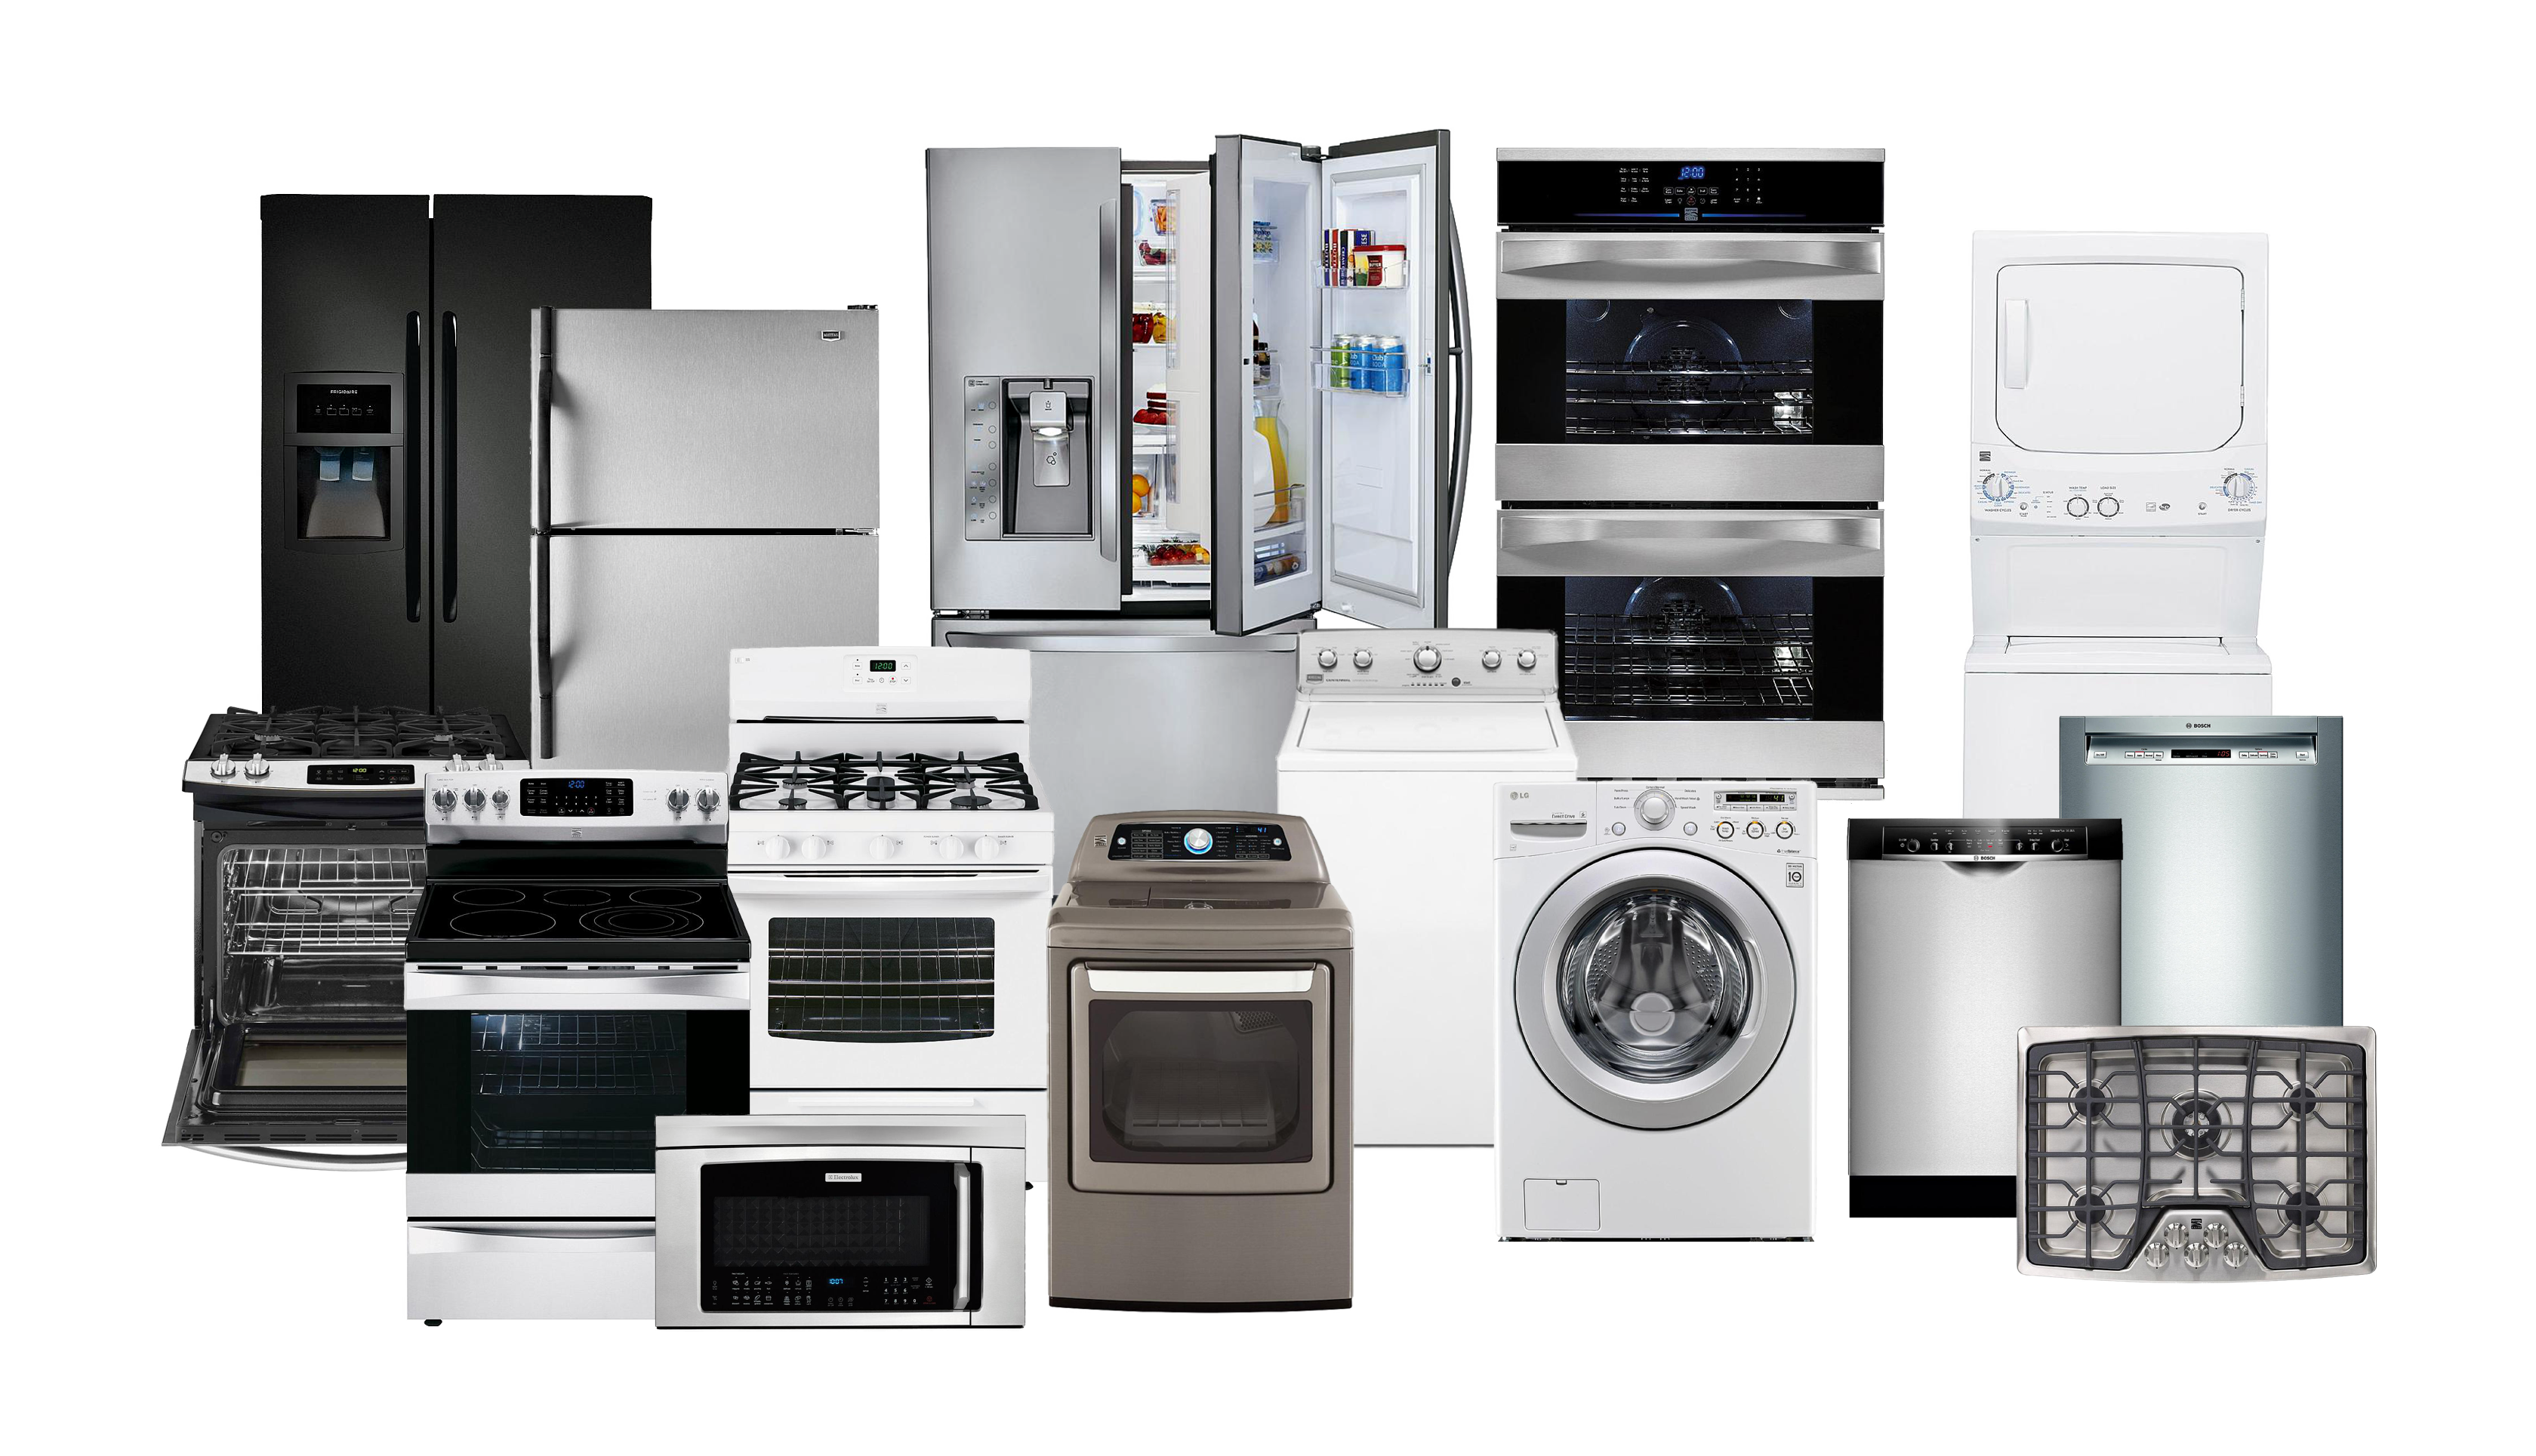
\includegraphics[width=8em]{img/appliances.png} &
			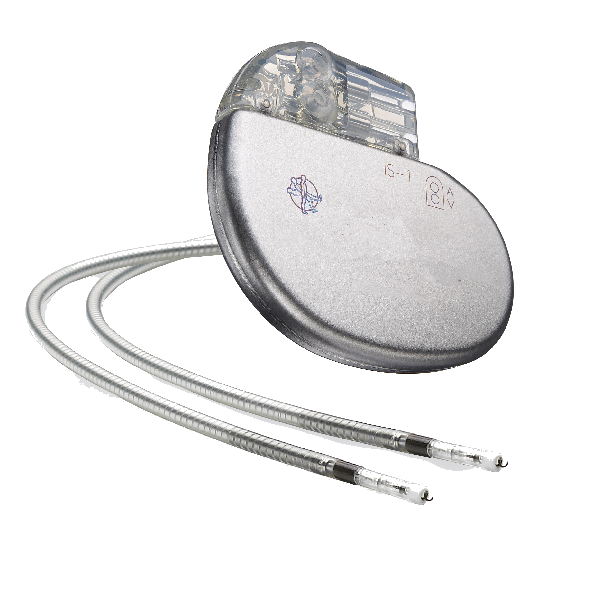
\includegraphics[width=8em]{img/Permanent-Pacemaker.png} &
			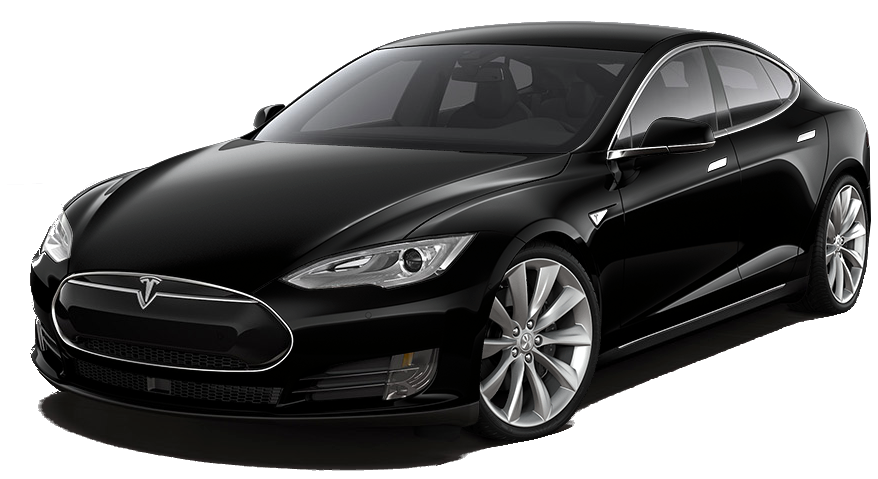
\includegraphics[width=8em]{img/must_diagonaal1.png} \\
			\tiny{\textbf{Cellphones}} &
			\tiny{\textbf{Appliances}} &
			\tiny{\textbf{Medical Devices}} &
			\tiny{\textbf{Transportation}}
		\end{tabular}
	\end{frame}
%%%%%%%%%%%%%%%%%%%%%%%%%%%%%%%%%%%%%%%%%%%%%%%%%%%%%%%%%%%%%%%%%%%%%%%%%%%%%%%%%%%%	
	

	
%%%%%%%%%%%%%%%%%%%%%%%%%%%%%%%%%%%%%%%%%%%%%%%%%%%%%%%%%%%%%%%%%%%%%%%%%%%%%%%%%%%%
% Where Can You Find Embedded Systems?
%%%%%%%%%%%%%%%%%%%%%%%%%%%%%%%%%%%%%%%%%%%%%%%%%%%%%%%%%%%%%%%%%%%%%%%%%%%%%%%%%%%%	
	\begin{frame}{Where Can You Find Embedded Systems?}
	\centering
		\begin{tabular}{c c c c}		
			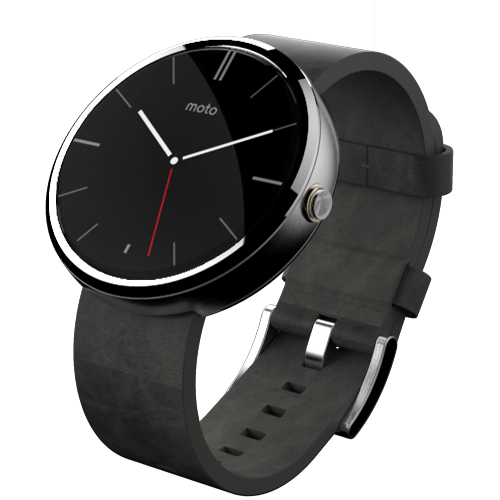
\includegraphics[width=8em]{img/Motorola_Moto_360_Minimal_Watch_Face.png} &
			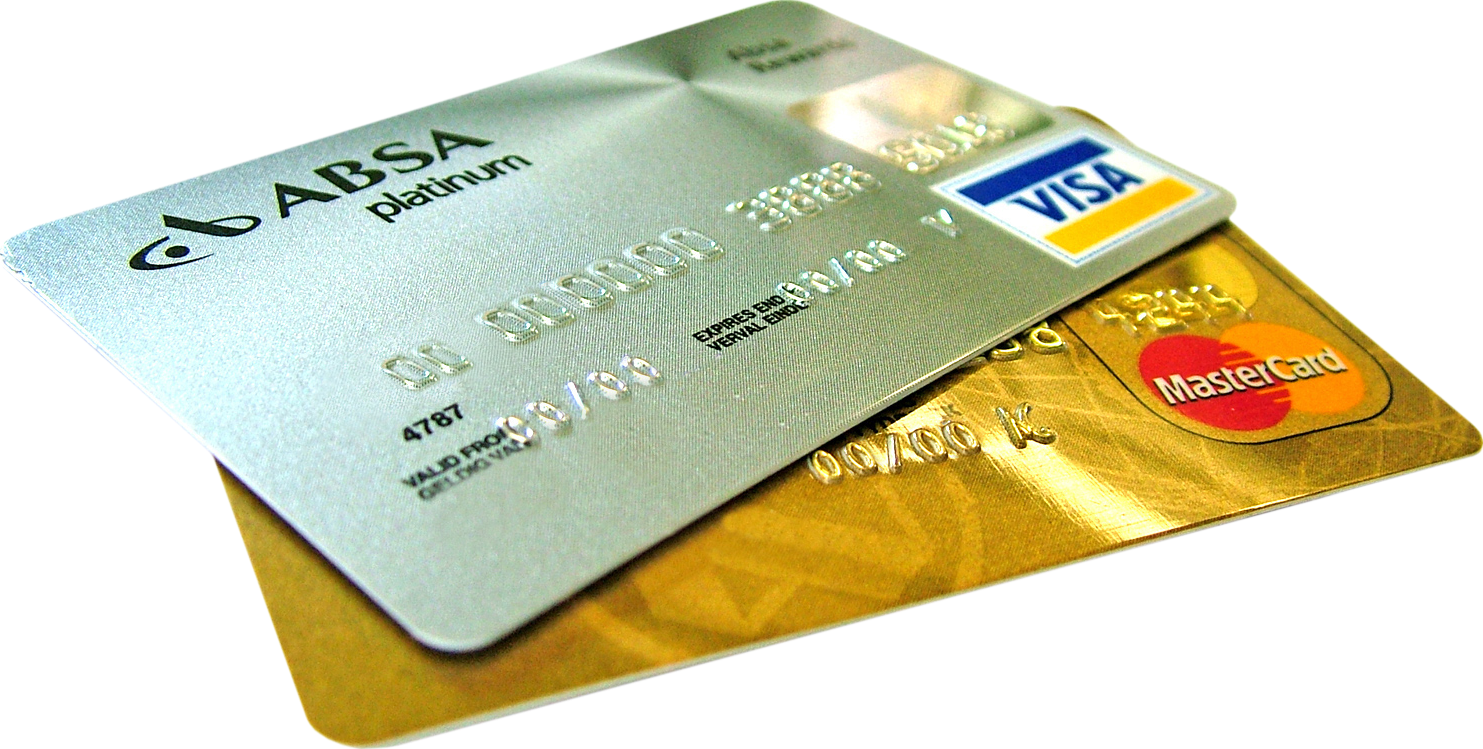
\includegraphics[width=8em]{img/creditcards.png} &
			
\includegraphics[width=8em]{img/IMG_0198} &
			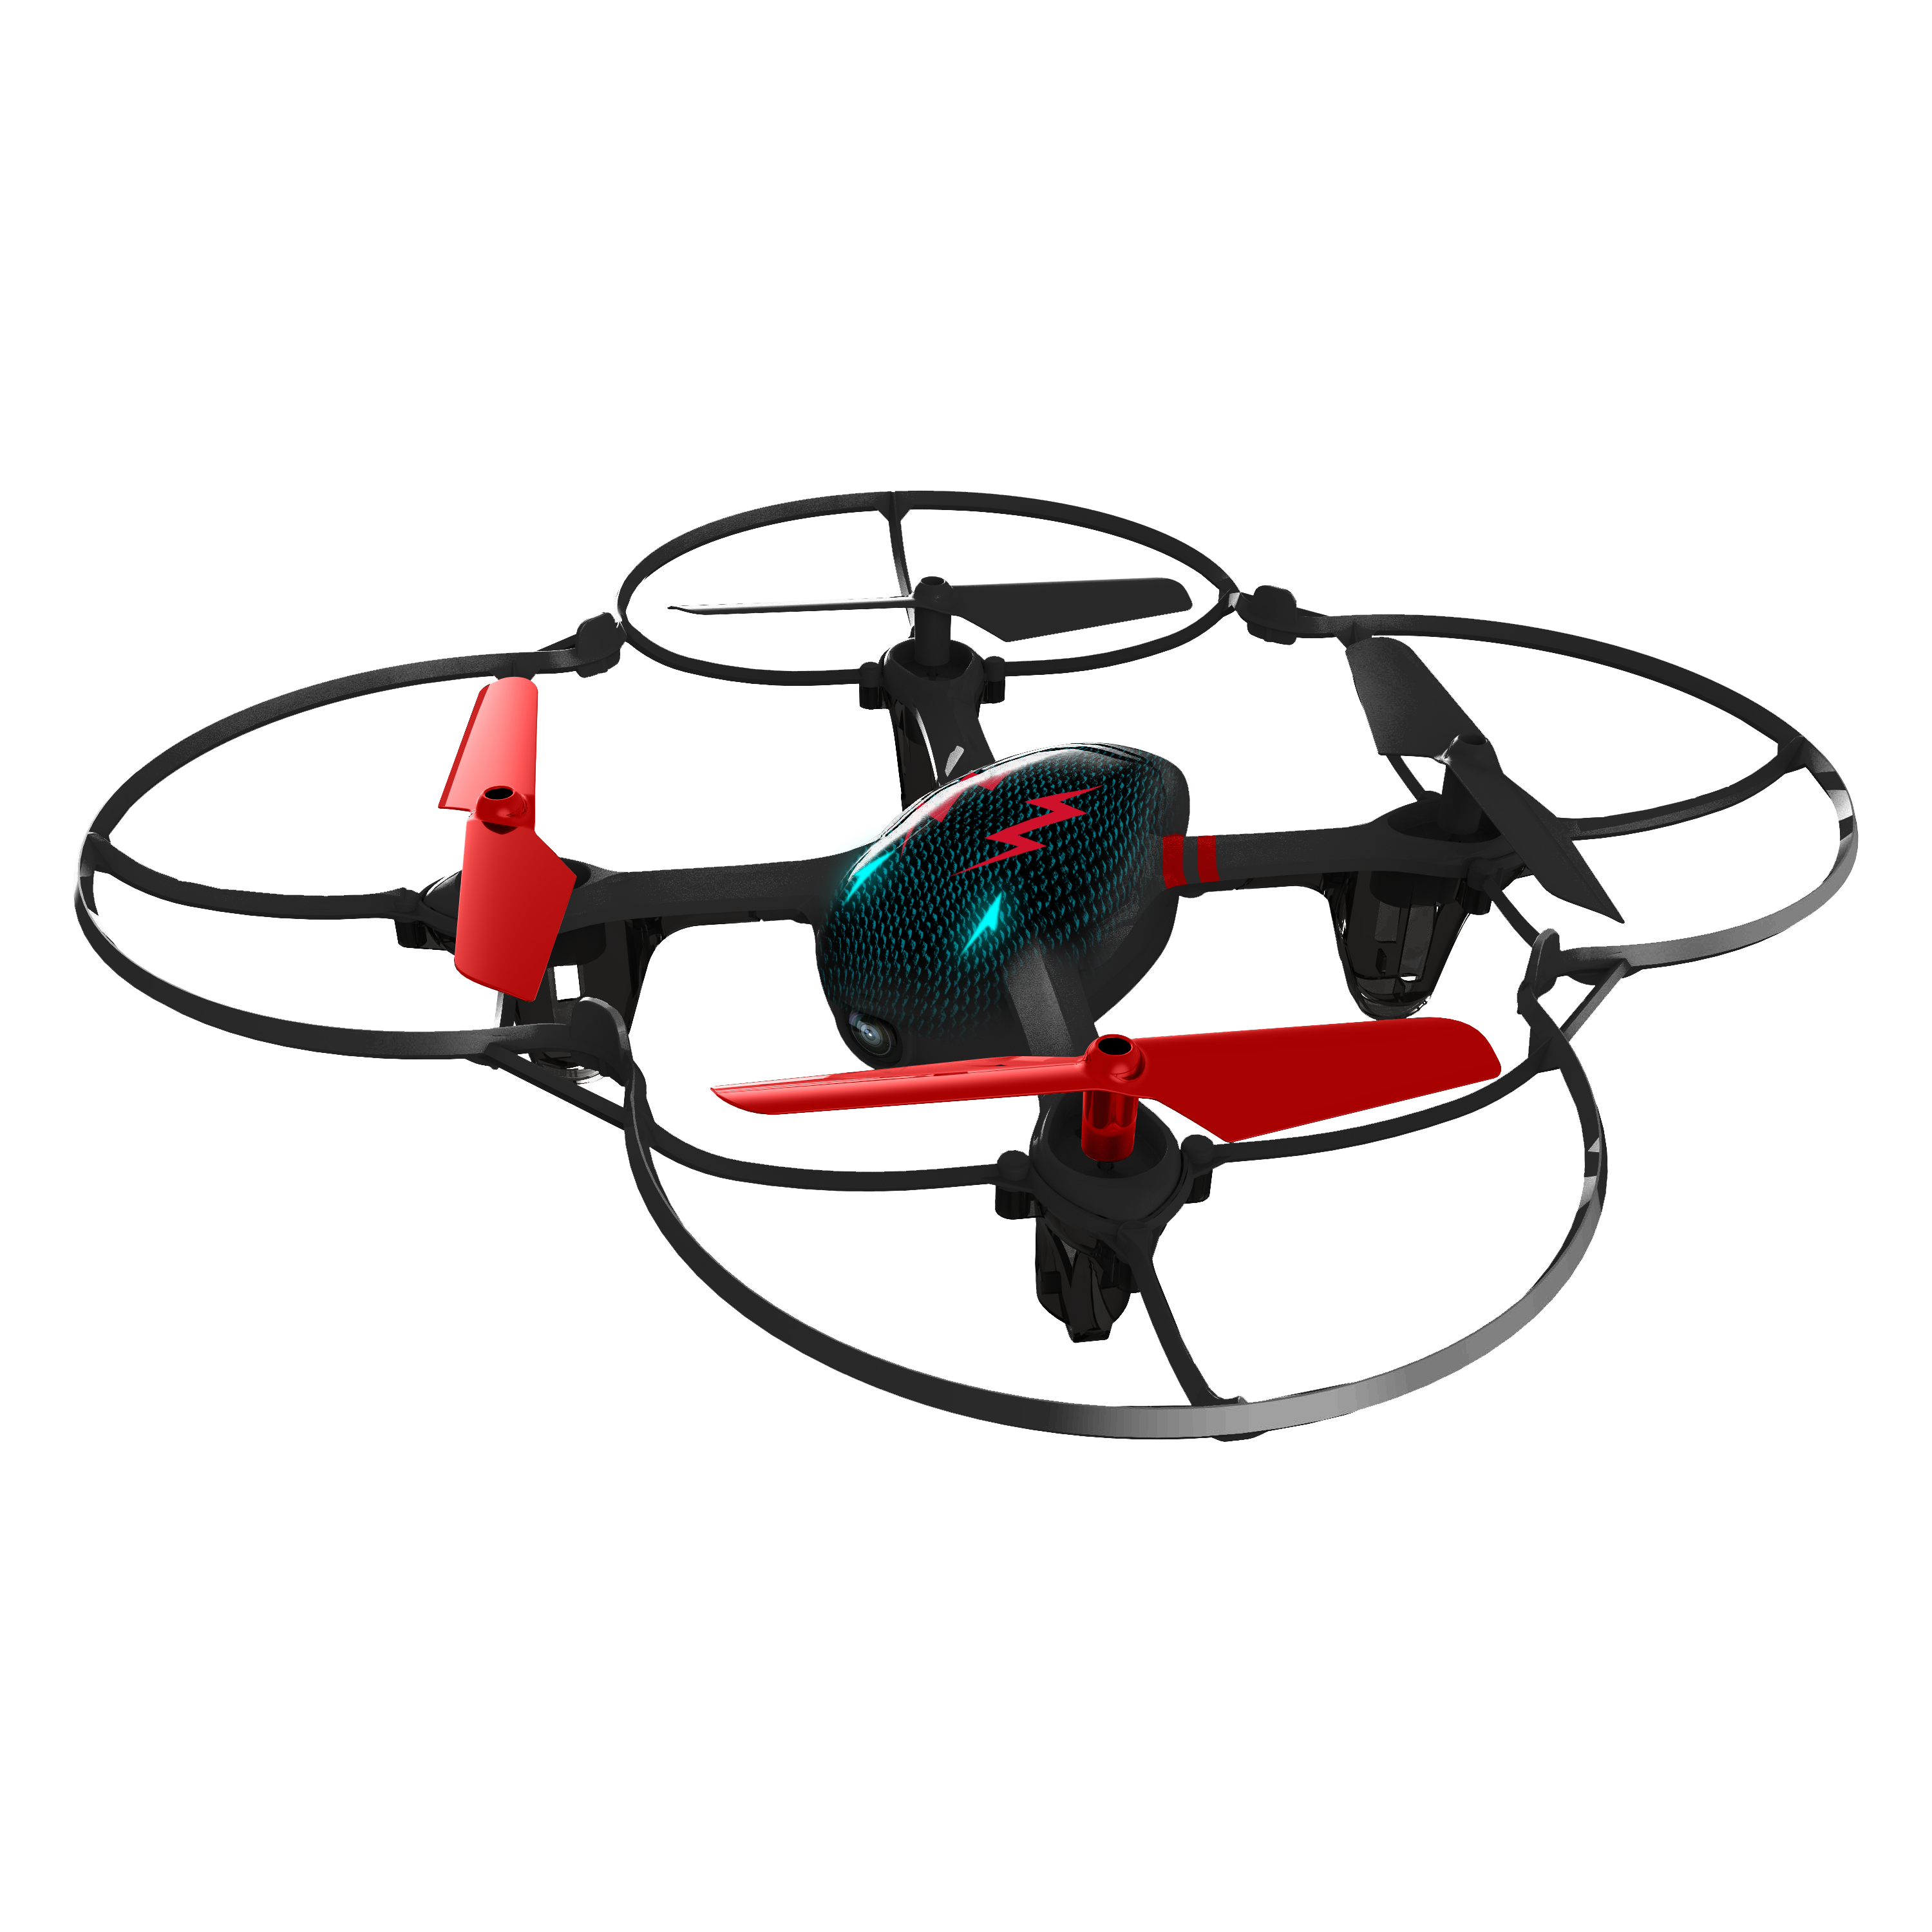
\includegraphics[width=8em]{img/electro_max_eye_720p_video_drone_angle_left} \\
			\tiny{\textbf{Watches}} &
			\tiny{\textbf{Credit Cards}} &
			\tiny{\textbf{Pets}} &
			\tiny{\textbf{Toys}}
		\end{tabular}
		\newline		
		
		Let's just say that embedded systems are everywhere.
	\end{frame}
%%%%%%%%%%%%%%%%%%%%%%%%%%%%%%%%%%%%%%%%%%%%%%%%%%%%%%%%%%%%%%%%%%%%%%%%%%%%%%%%%%%%	



%%%%%%%%%%%%%%%%%%%%%%%%%%%%%%%%%%%%%%%%%%%%%%%%%%%%%%%%%%%%%%%%%%%%%%%%%%%%%%%%%%%%
% Two Types of Embedded Systems
%%%%%%%%%%%%%%%%%%%%%%%%%%%%%%%%%%%%%%%%%%%%%%%%%%%%%%%%%%%%%%%%%%%%%%%%%%%%%%%%%%%%
\begin{frame}{Kinds of Embedded Systems}
\textbf{Embedded Systems} \\
\textit{Simple:} made of electronics, no processor or control software. \\ 
\textit{Complex:} has one or more processors along with control software. \\
\vspace{2em}
\textbf{Embedded Computer Systems} \\
A special-purpose computer system designed to perform a set of tasks without the user's knowledge of its existence. \\
\vspace{2em}
I like the distinction that an embedded system is \textbf{purpose-built}.
\end{frame}  
%%%%%%%%%%%%%%%%%%%%%%%%%%%%%%%%%%%%%%%%%%%%%%%%%%%%%%%%%%%%%%%%%%%%%%%%%%%%%%%%%%%%	  
  
  
  
%%%%%%%%%%%%%%%%%%%%%%%%%%%%%%%%%%%%%%%%%%%%%%%%%%%%%%%%%%%%%%%%%%%%%%%%%%%%%%%%%%%%
% Simple Embedded System Diagram
%%%%%%%%%%%%%%%%%%%%%%%%%%%%%%%%%%%%%%%%%%%%%%%%%%%%%%%%%%%%%%%%%%%%%%%%%%%%%%%%%%%%
	\begin{frame}{Framework For a Simple Embedded System}
	\begin{center}		
		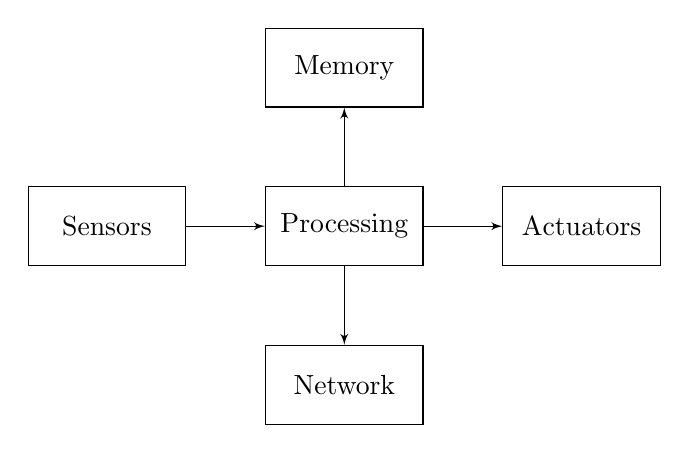
\begin{tikzpicture}[auto, node distance=2cm,>=latex']
			\tikzset{block/.style= {draw, rectangle, align=center,minimum width=2cm,minimum height=1cm},
        rblock/.style={draw, shape=rectangle,rounded corners=1em,align=center,minimum width=2cm,minimum height=1cm},
        input/.style={ % requires library shapes.geometric
        draw,
        trapezium,
        trapezium left angle=60,
        trapezium right angle=120,
        minimum width=2cm,
        align=center,
        minimum height=1cm
    },
        }

			\node [block](sensors) {Sensors};
			\node [block, right=1cm of sensors] (processing) {Processing};
			\node [block, above=1cm of processing] (memory) {Memory};
			\node [block, below=1cm of processing] (network) {Network};
			\node [block, right=1cm of processing] (actuators) {Actuators};
			
			\path[draw,->] (sensors) edge (processing);
			\path[draw,->] (processing) edge (actuators);
			\path[draw,->] (processing) edge (memory);
			\path[draw,->] (processing) edge (network);

		\end{tikzpicture}
	\end{center}	
	\end{frame}
%%%%%%%%%%%%%%%%%%%%%%%%%%%%%%%%%%%%%%%%%%%%%%%%%%%%%%%%%%%%%%%%%%%%%%%%%%%%%%%%%%%%	
	
	
	
\section{An Example of An Automotive Embedded System}	
	
	
  
%%%%%%%%%%%%%%%%%%%%%%%%%%%%%%%%%%%%%%%%%%%%%%%%%%%%%%%%%%%%%%%%%%%%%%%%%%%%%%%%%%%%
% Spark Control in an ICE
%%%%%%%%%%%%%%%%%%%%%%%%%%%%%%%%%%%%%%%%%%%%%%%%%%%%%%%%%%%%%%%%%%%%%%%%%%%%%%%%%%%%
	\begin{frame}{Example: Spark Control in an Internal Combustion Engine}
	\vspace{1em}
	\begin{columns}
	\begin{column}{0.6\textwidth}
	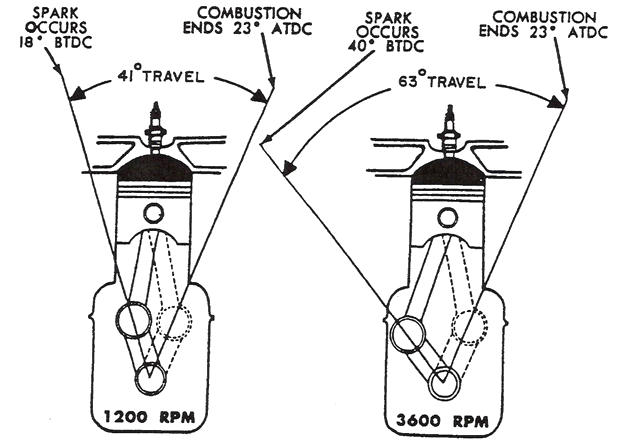
\includegraphics[width=0.95\textwidth,keepaspectratio]{img/LeanAdvance.png}
	\end{column}
	\begin{column}{0.4\textwidth}
	\textbf{Problem:} We need to generate a spark when the piston is at a particular position. \\
	\vspace{1em}
	\textbf{Complication:} The spark position is not a constant! It changes as a function of engine speed and engine load.
	\end{column}
	\end{columns}
	\vspace{1em}
	\begin{footnotesize}http://www.preludepower.com/forums/showthread.php?t=252042\end{footnotesize}
	\end{frame}	  
%%%%%%%%%%%%%%%%%%%%%%%%%%%%%%%%%%%%%%%%%%%%%%%%%%%%%%%%%%%%%%%%%%%%%%%%%%%%%%%%%%%%  
  
  
  
%%%%%%%%%%%%%%%%%%%%%%%%%%%%%%%%%%%%%%%%%%%%%%%%%%%%%%%%%%%%%%%%%%%%%%%%%%%%%%%%%%%%
% Spark Control in an ICE
%%%%%%%%%%%%%%%%%%%%%%%%%%%%%%%%%%%%%%%%%%%%%%%%%%%%%%%%%%%%%%%%%%%%%%%%%%%%%%%%%%%%
\begin{frame}[t]{Example: Spark Control in an Internal Combustion Engine}
Back in the (dark) days of purely mechanical systems, we have the distributor.
\begin{figure}
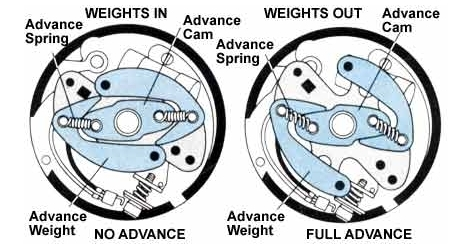
\includegraphics[scale=0.70]{img/3-8-ignition_clip_image005.jpg}
\caption{http://www.scuderiatopolino.com/3-8-ignition.php}
\end{figure}
\href{https://www.youtube.com/watch?v=RcmkbQVPz9E}{Mechanical Spark Advance In Action}
\end{frame}
%%%%%%%%%%%%%%%%%%%%%%%%%%%%%%%%%%%%%%%%%%%%%%%%%%%%%%%%%%%%%%%%%%%%%%%%%%%%%%%%%%%%



%%%%%%%%%%%%%%%%%%%%%%%%%%%%%%%%%%%%%%%%%%%%%%%%%%%%%%%%%%%%%%%%%%%%%%%%%%%%%%%%%%%%
% Spark Control in an ICE
%%%%%%%%%%%%%%%%%%%%%%%%%%%%%%%%%%%%%%%%%%%%%%%%%%%%%%%%%%%%%%%%%%%%%%%%%%%%%%%%%%%%
	\begin{frame}{Example: Spark Control in an Internal Combustion Engine}
		Today, we use a simple embedded control system:
		\vspace{2em}		
		\begin{columns}
		\begin{column}{0.45\textwidth}		
		{\bf Inputs (Sensors):}
		\begin{itemize}
			\item Crankshaft position / speed
			\item Throttle position
		\end{itemize}
		
		{\bf Processing:}
		\begin{itemize}
			\item A 2-D lookup table of spark time vs. \\
			engine speed and throttle position
		\end{itemize}
		
		{\bf Outputs (Actuators):}
		\begin{itemize}
			\item Signal to close spark contact
		\end{itemize}
		\end{column}
		\begin{column}{0.5\textwidth}
		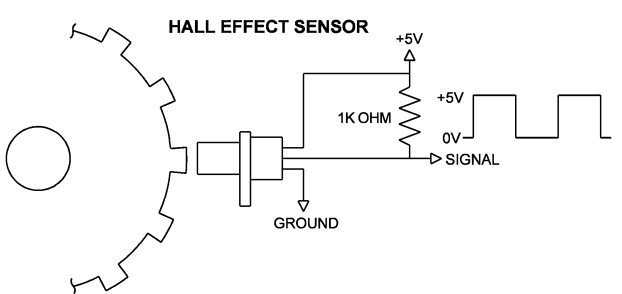
\includegraphics[width=1.0\textwidth]{img/CKP_Sensor_Waveforms.png}
		\end{column}
		\end{columns}	
		\begin{flushright}
		\begin{tiny}https://nwmobilemechanicdotcom.wordpress.com/2012/11/28/the-hall-effect-crankshaft-sensor/\end{tiny}
		\end{flushright}
	\end{frame}
%%%%%%%%%%%%%%%%%%%%%%%%%%%%%%%%%%%%%%%%%%%%%%%%%%%%%%%%%%%%%%%%%%%%%%%%%%%%%%%%%%%%



%%%%%%%%%%%%%%%%%%%%%%%%%%%%%%%%%%%%%%%%%%%%%%%%%%%%%%%%%%%%%%%%%%%%%%%%%%%%%%%%%%%%
% Embedded Systems Challenges
%%%%%%%%%%%%%%%%%%%%%%%%%%%%%%%%%%%%%%%%%%%%%%%%%%%%%%%%%%%%%%%%%%%%%%%%%%%%%%%%%%%%
\begin{frame}{Challenges in Designing and Programming Embedded Systems}
Designers of embedded computer systems face some challenges: \\
\begin{itemize}
\item Limited processing power and memory
\item Potentially harsh operating environment
\item Hardware and platform variability
\item Limited or non-existent user interface
\item Minimal or non-existent operating system and APIs
\item Hard to access, service, and upgrade once they are deployed
\end{itemize}
\end{frame}
%%%%%%%%%%%%%%%%%%%%%%%%%%%%%%%%%%%%%%%%%%%%%%%%%%%%%%%%%%%%%%%%%%%%%%%%%%%%%%%%%%%%



\section{Smartphones as Embedded Systems}	



%%%%%%%%%%%%%%%%%%%%%%%%%%%%%%%%%%%%%%%%%%%%%%%%%%%%%%%%%%%%%%%%%%%%%%%%%%%%%%%%%%%%
% Inside a Smartphone
%%%%%%%%%%%%%%%%%%%%%%%%%%%%%%%%%%%%%%%%%%%%%%%%%%%%%%%%%%%%%%%%%%%%%%%%%%%%%%%%%%%%
	\begin{frame}{Inside a Smartphone}
		
		Since we're going to be using Android in this course, let's take a brief look
		inside my favourite phone, the {\bf OnePlus One}.
		
		\href{https://www.ifixit.com/Teardown/OnePlus+One+Teardown/26484}{https://www.ifixit.com/Teardown/OnePlus+One+Teardown/26484}
		
		\vspace{1em}		
		
		\centering
		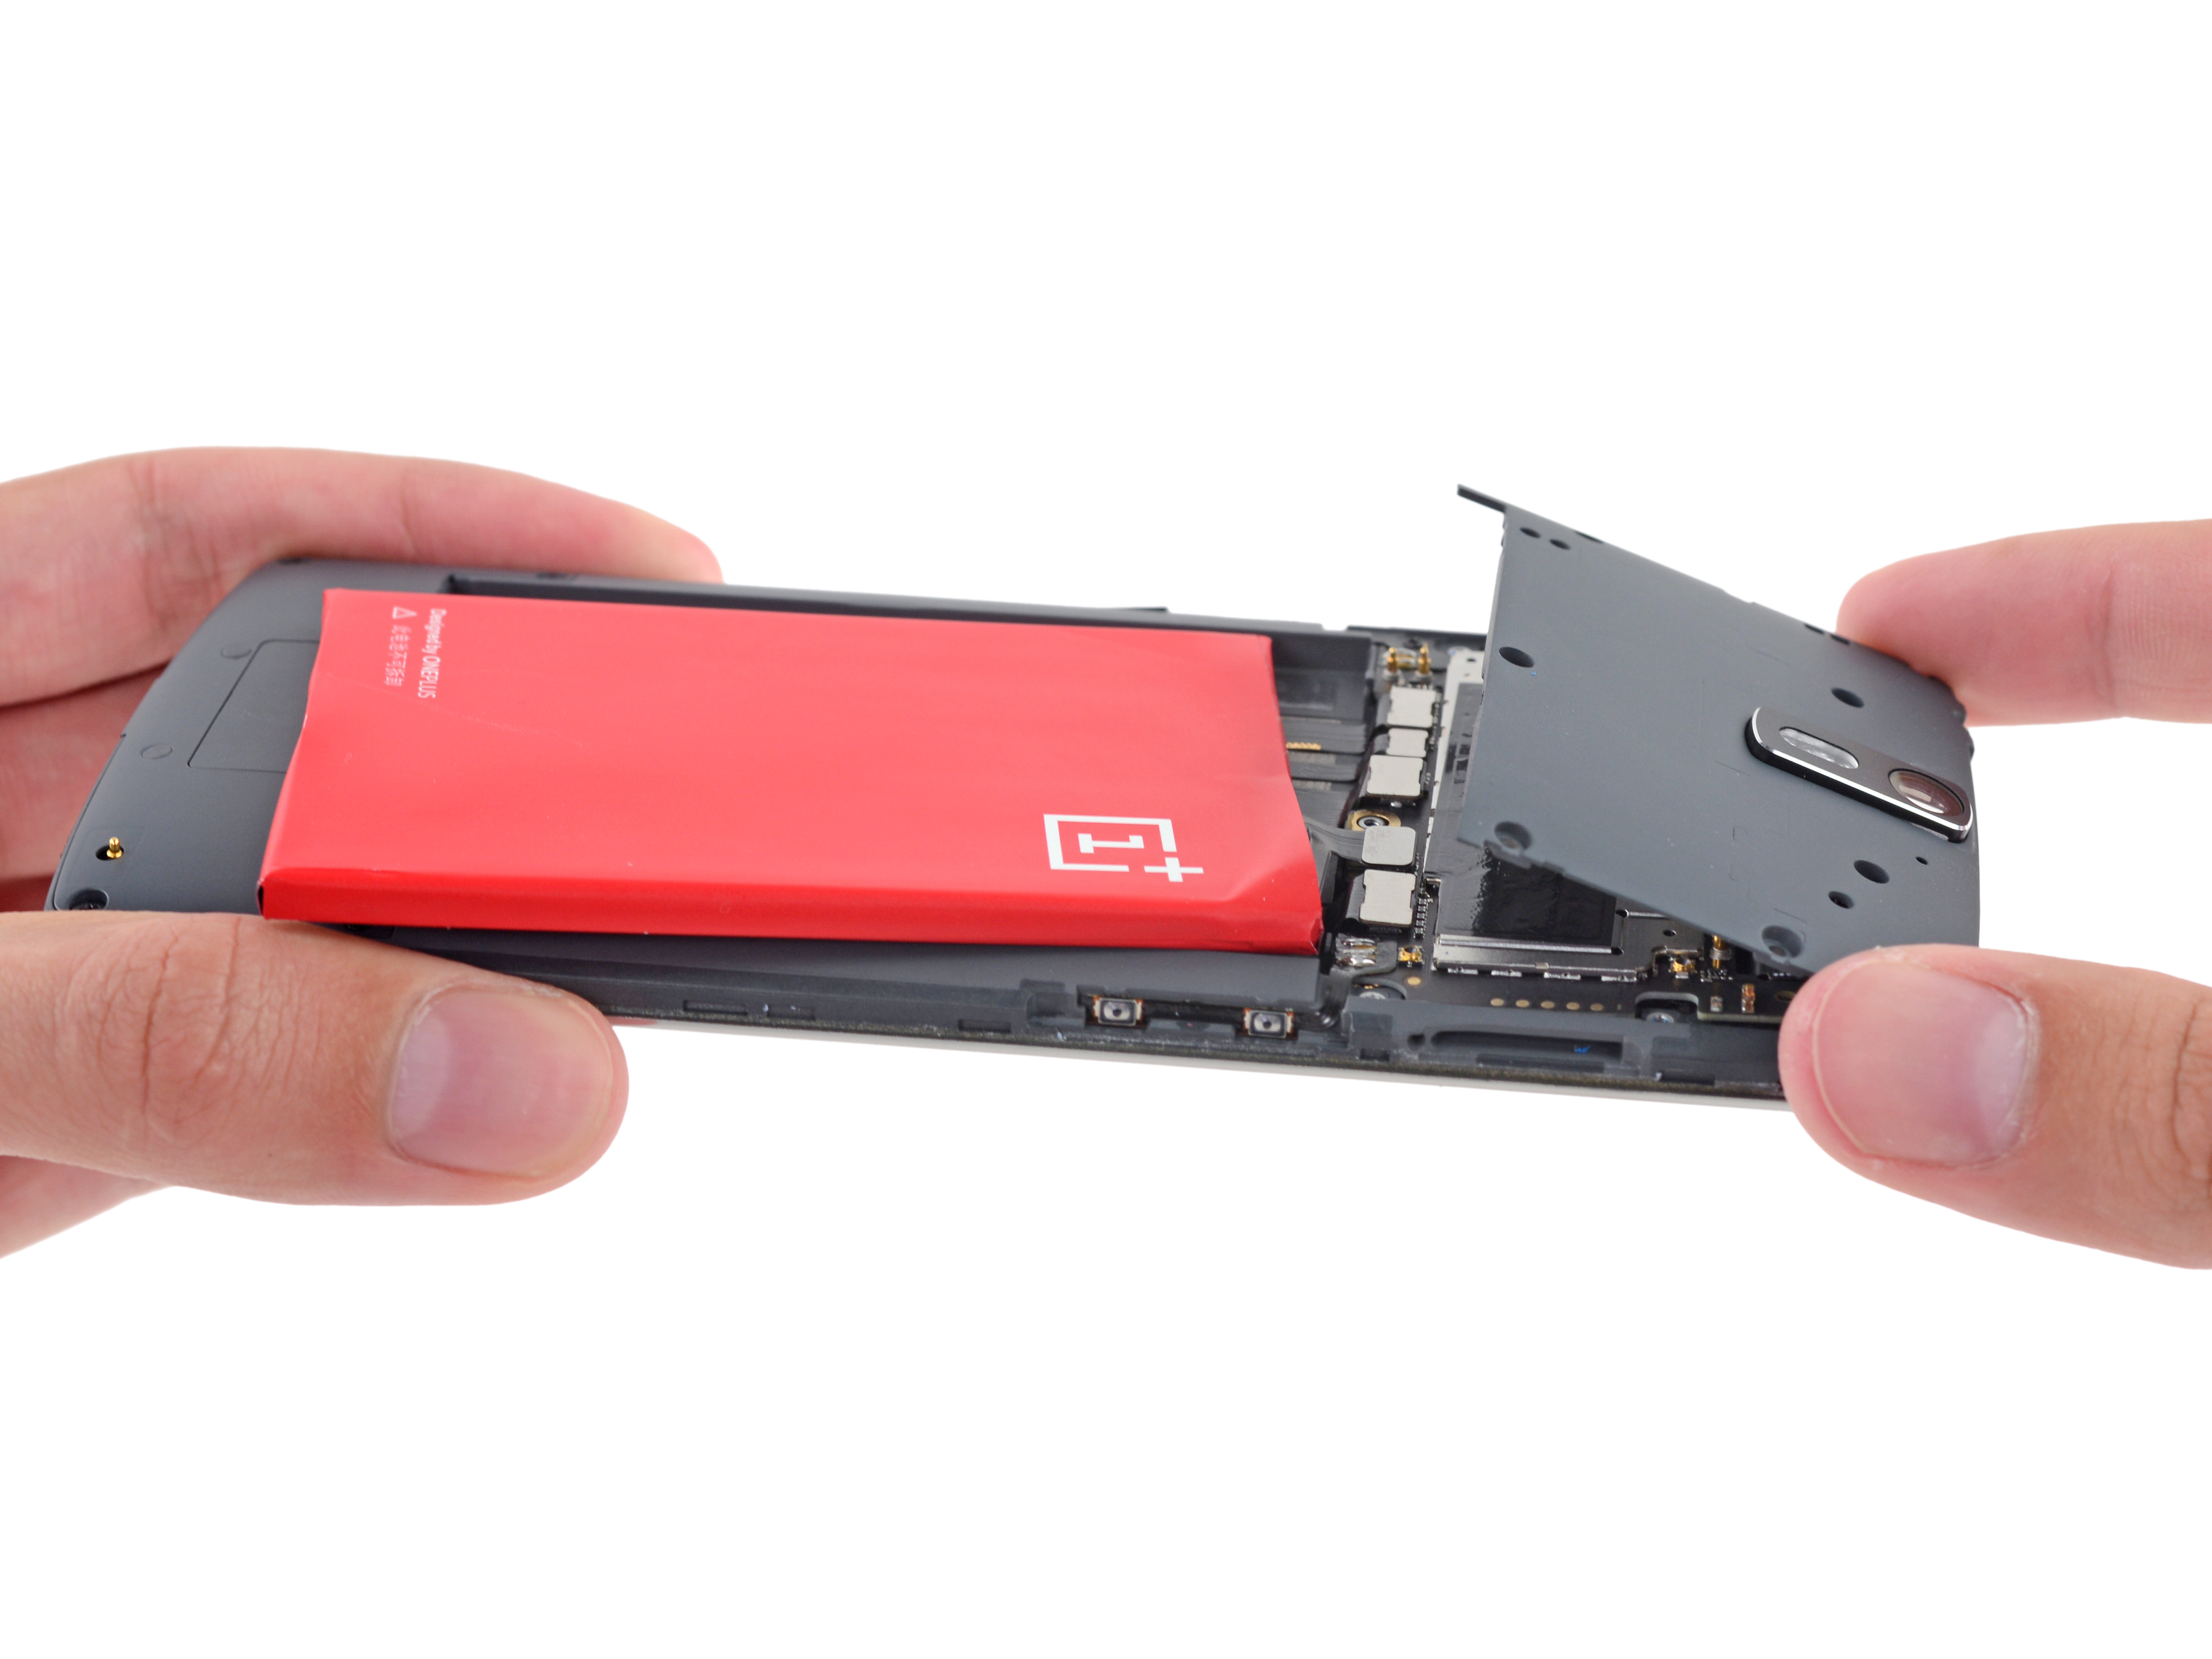
\includegraphics[width=\textwidth,height=5cm,keepaspectratio]{img/WJweKyYej2qtrc4m.png}
			
	\end{frame}
%%%%%%%%%%%%%%%%%%%%%%%%%%%%%%%%%%%%%%%%%%%%%%%%%%%%%%%%%%%%%%%%%%%%%%%%%%%%%%%%%%%%



%%%%%%%%%%%%%%%%%%%%%%%%%%%%%%%%%%%%%%%%%%%%%%%%%%%%%%%%%%%%%%%%%%%%%%%%%%%%%%%%%%%%
% Inside a Smartphone
%%%%%%%%%%%%%%%%%%%%%%%%%%%%%%%%%%%%%%%%%%%%%%%%%%%%%%%%%%%%%%%%%%%%%%%%%%%%%%%%%%%%	
	\begin{frame}{Inside a Smartphone}
		We have two cameras (sensors) sitting at the top of the phone.
		\begin{figure}[b]		
		\centering
		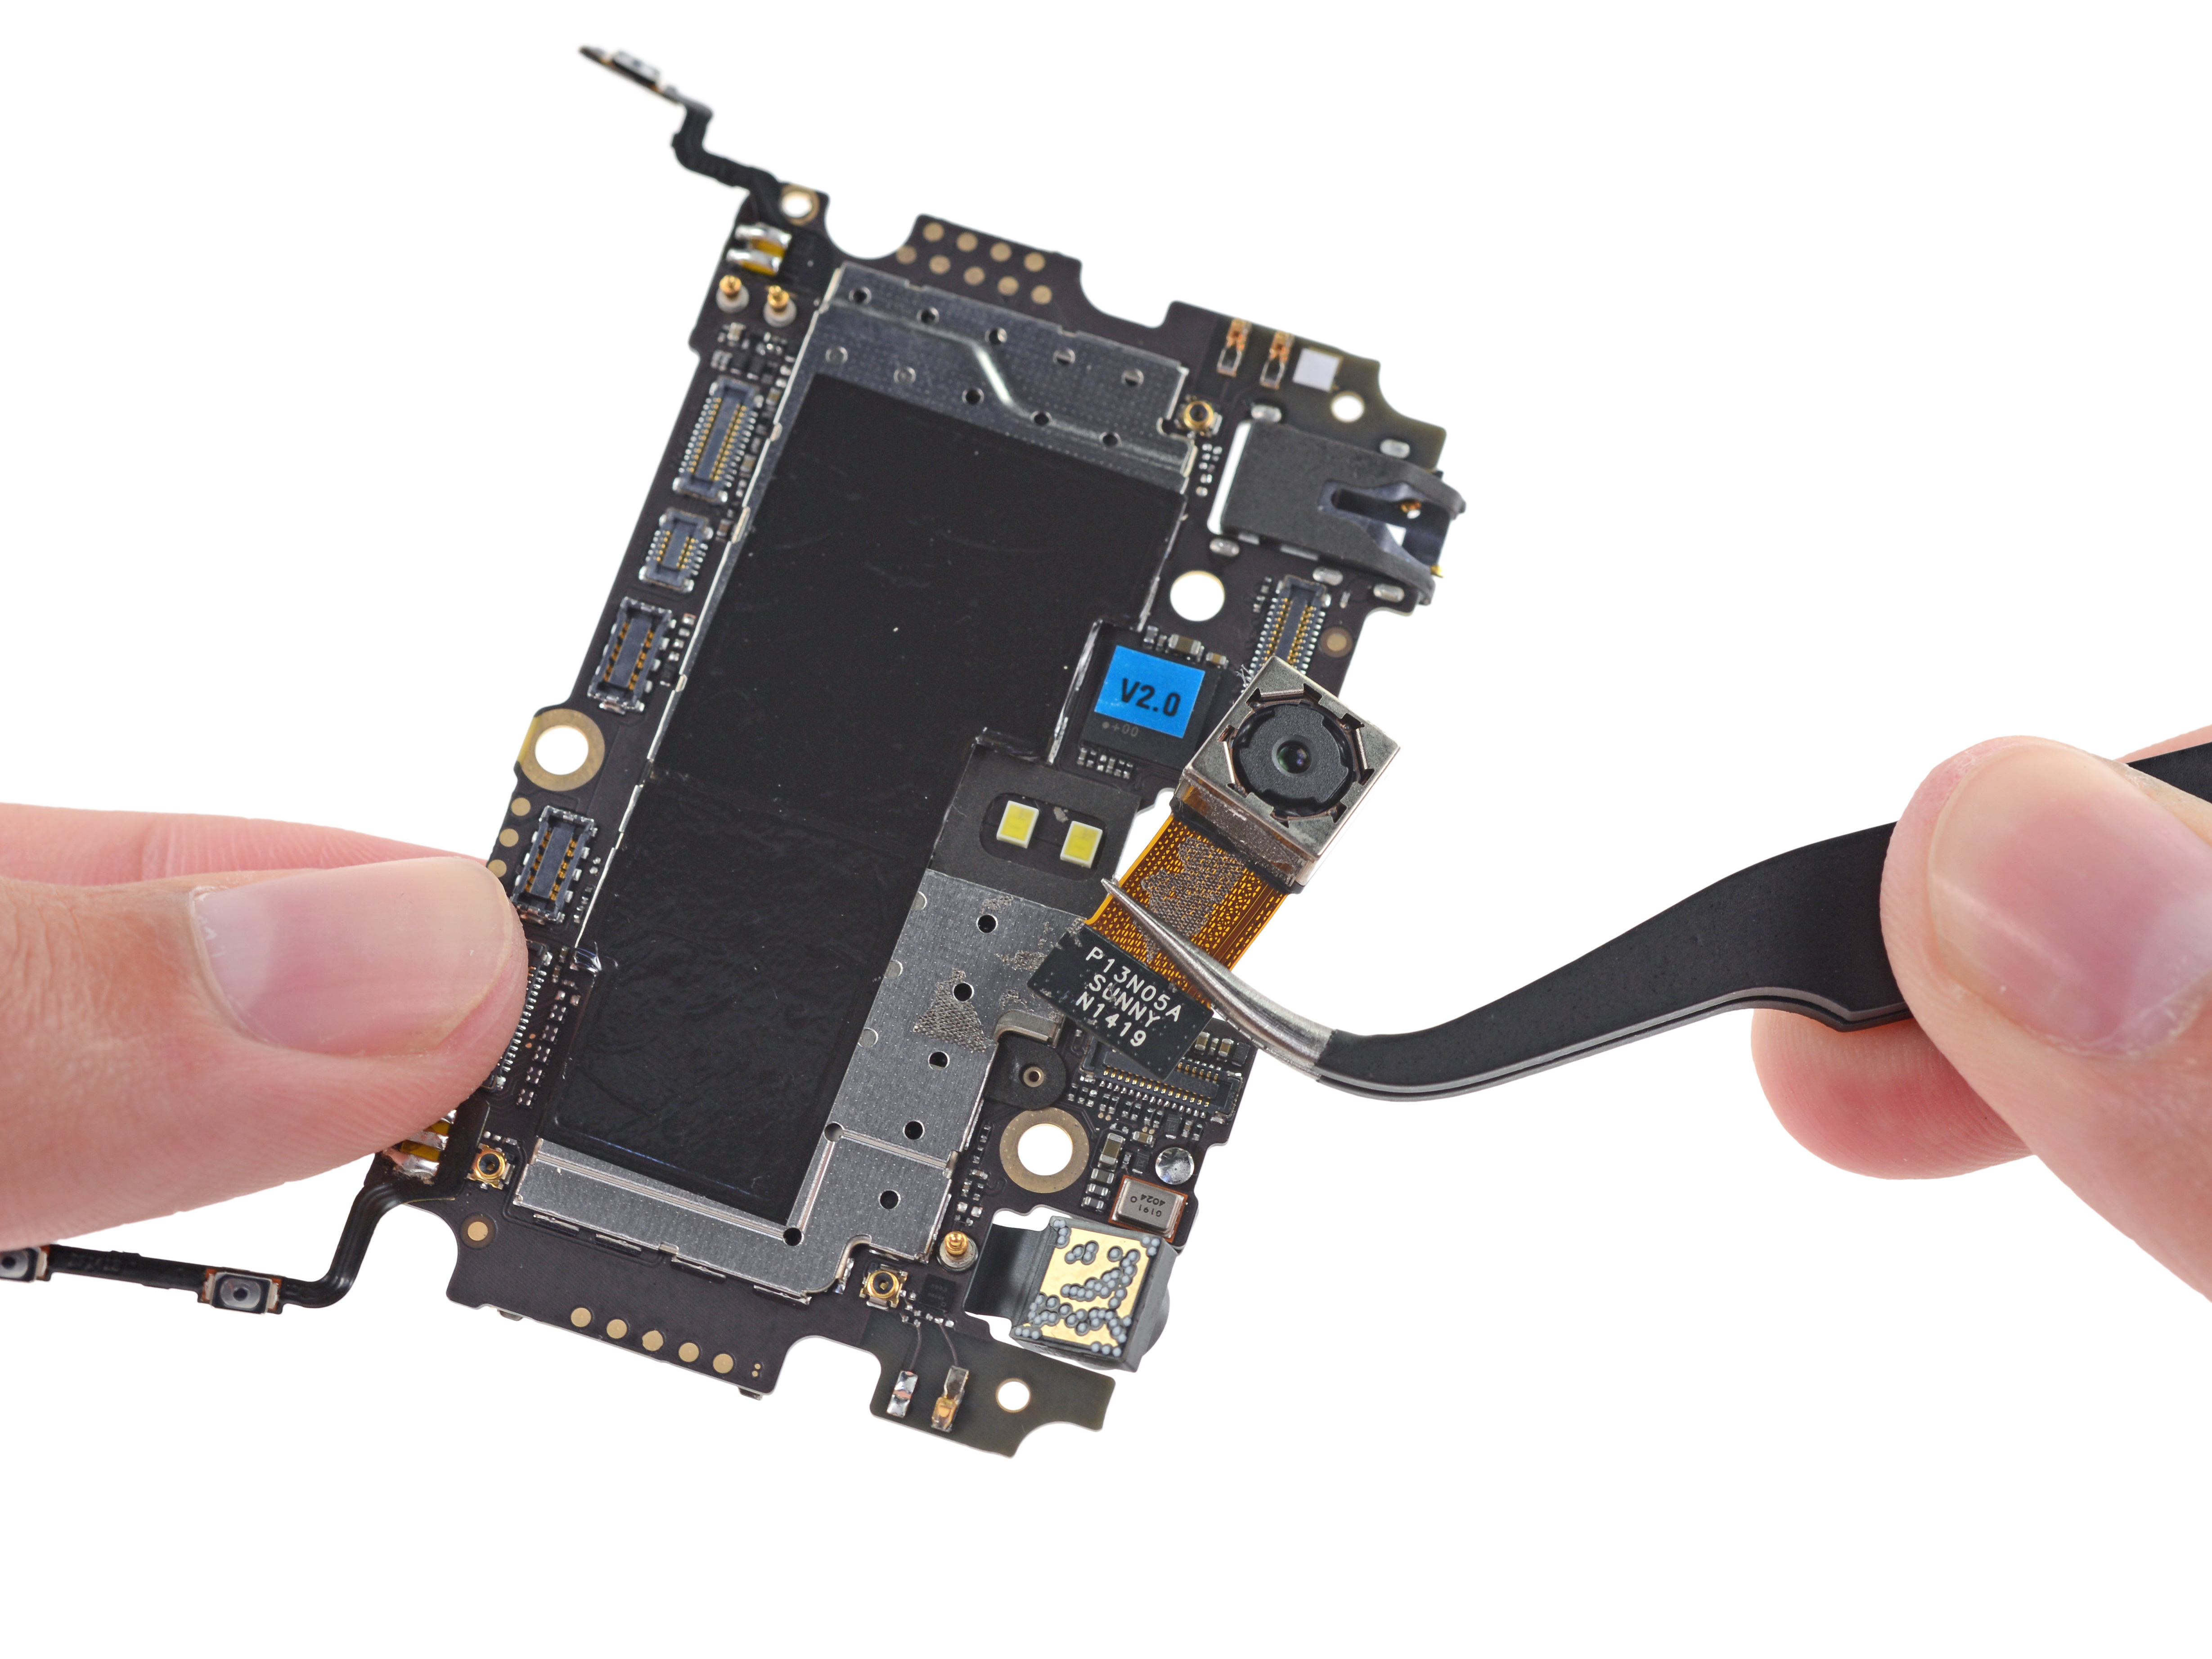
\includegraphics[width=\textwidth,height=6cm,keepaspectratio]{img/SuhLygXH4QXdDMEm.png}
		\end{figure}
	\end{frame}
%%%%%%%%%%%%%%%%%%%%%%%%%%%%%%%%%%%%%%%%%%%%%%%%%%%%%%%%%%%%%%%%%%%%%%%%%%%%%%%%%%%%



%%%%%%%%%%%%%%%%%%%%%%%%%%%%%%%%%%%%%%%%%%%%%%%%%%%%%%%%%%%%%%%%%%%%%%%%%%%%%%%%%%%%
% Inside a Smartphone
%%%%%%%%%%%%%%%%%%%%%%%%%%%%%%%%%%%%%%%%%%%%%%%%%%%%%%%%%%%%%%%%%%%%%%%%%%%%%%%%%%%%
	\begin{frame}{Inside a Smartphone}
		\begin{flushleft}The motherboard is crammed full of embedded components...\end{flushleft}
		\begin{columns}
		\begin{column}{0.55\textwidth}	
		\centering
		\includegraphics[width=1.0\textwidth,keepaspectratio]{img/wIp5pQj4movpelpR_cut.png}	
		\end{column}
		\begin{column}{0.45\textwidth}
		\centering		
		\begin{footnotesize}
		\begin{itemize}
		\setlength\itemsep{1em}
		\item[\textcolor{red}{$\bullet$}] Samsung K3QF7F70DM-QGCF 3 GB LPDDR3 RAM; Qualcomm Snapdragon 801 likely layered beneath
		\item[\textcolor{orange}{$\bullet$}] Qualcomm WCD9320 Audio Codec
		\item[\textcolor{yellow}{$\bullet$}] AGD2 2402 WX9DR (likely gyroscope)
		\item[\textcolor{green}{$\bullet$}] Qualcomm PM8941 and PM8841 Power Management ICs Quick Charge 2.0 capable
		\end{itemize}
		\end{footnotesize}
		\end{column}
		\end{columns}
	\end{frame}  
%%%%%%%%%%%%%%%%%%%%%%%%%%%%%%%%%%%%%%%%%%%%%%%%%%%%%%%%%%%%%%%%%%%%%%%%%%%%%%%%%%%%



%%%%%%%%%%%%%%%%%%%%%%%%%%%%%%%%%%%%%%%%%%%%%%%%%%%%%%%%%%%%%%%%%%%%%%%%%%%%%%%%%%%%
% Inside a Smartphone
%%%%%%%%%%%%%%%%%%%%%%%%%%%%%%%%%%%%%%%%%%%%%%%%%%%%%%%%%%%%%%%%%%%%%%%%%%%%%%%%%%%%
	\begin{frame}{Inside a Smartphone}
		\begin{flushleft}...on both sides\end{flushleft}
		\begin{columns}
		\begin{column}{0.55\textwidth}	
		\centering
		\includegraphics[width=1.0\textwidth,keepaspectratio]{img/FGcUA3hpq1ejhOQL_cut.png}	
		\end{column}
		\begin{column}{0.45\textwidth}
		\centering		
		\begin{footnotesize}
		\begin{itemize}
		\item[\textcolor{red}{$\bullet$}] Toshiba THGBMBG9D8KBAIG eMMC 5.0 64 GB Onboard Storage
		\item[\textcolor{orange}{$\bullet$}] Skyworks SKY77629-21 Power Amplifier Module
		\item[\textcolor{yellow}{$\bullet$}] Qualcomm WCN3680 802.11ac/FM/BT 4.0 Combo Chip
		\item[\textcolor{green}{$\bullet$}] Qualcomm WTR1625L RF Transceiver
		\item[\textcolor{blue}{$\bullet$}] Skyworks SKY85709 WLAN Front-End Module
		\item[\textcolor{purple}{$\bullet$}] Synaptics S3508A Touchscreen Controller
		\end{itemize}
		\end{footnotesize}
		\end{column}
		\end{columns}
	\end{frame}  
%%%%%%%%%%%%%%%%%%%%%%%%%%%%%%%%%%%%%%%%%%%%%%%%%%%%%%%%%%%%%%%%%%%%%%%%%%%%%%%%%%%%



%%%%%%%%%%%%%%%%%%%%%%%%%%%%%%%%%%%%%%%%%%%%%%%%%%%%%%%%%%%%%%%%%%%%%%%%%%%%%%%%%%%%
% Inside a Smartphone
%%%%%%%%%%%%%%%%%%%%%%%%%%%%%%%%%%%%%%%%%%%%%%%%%%%%%%%%%%%%%%%%%%%%%%%%%%%%%%%%%%%%
	\begin{frame}{Inside a Smartphone}
		The daughter-board at the bottom contains some actuators.
		\begin{figure}[b]
		\centering
		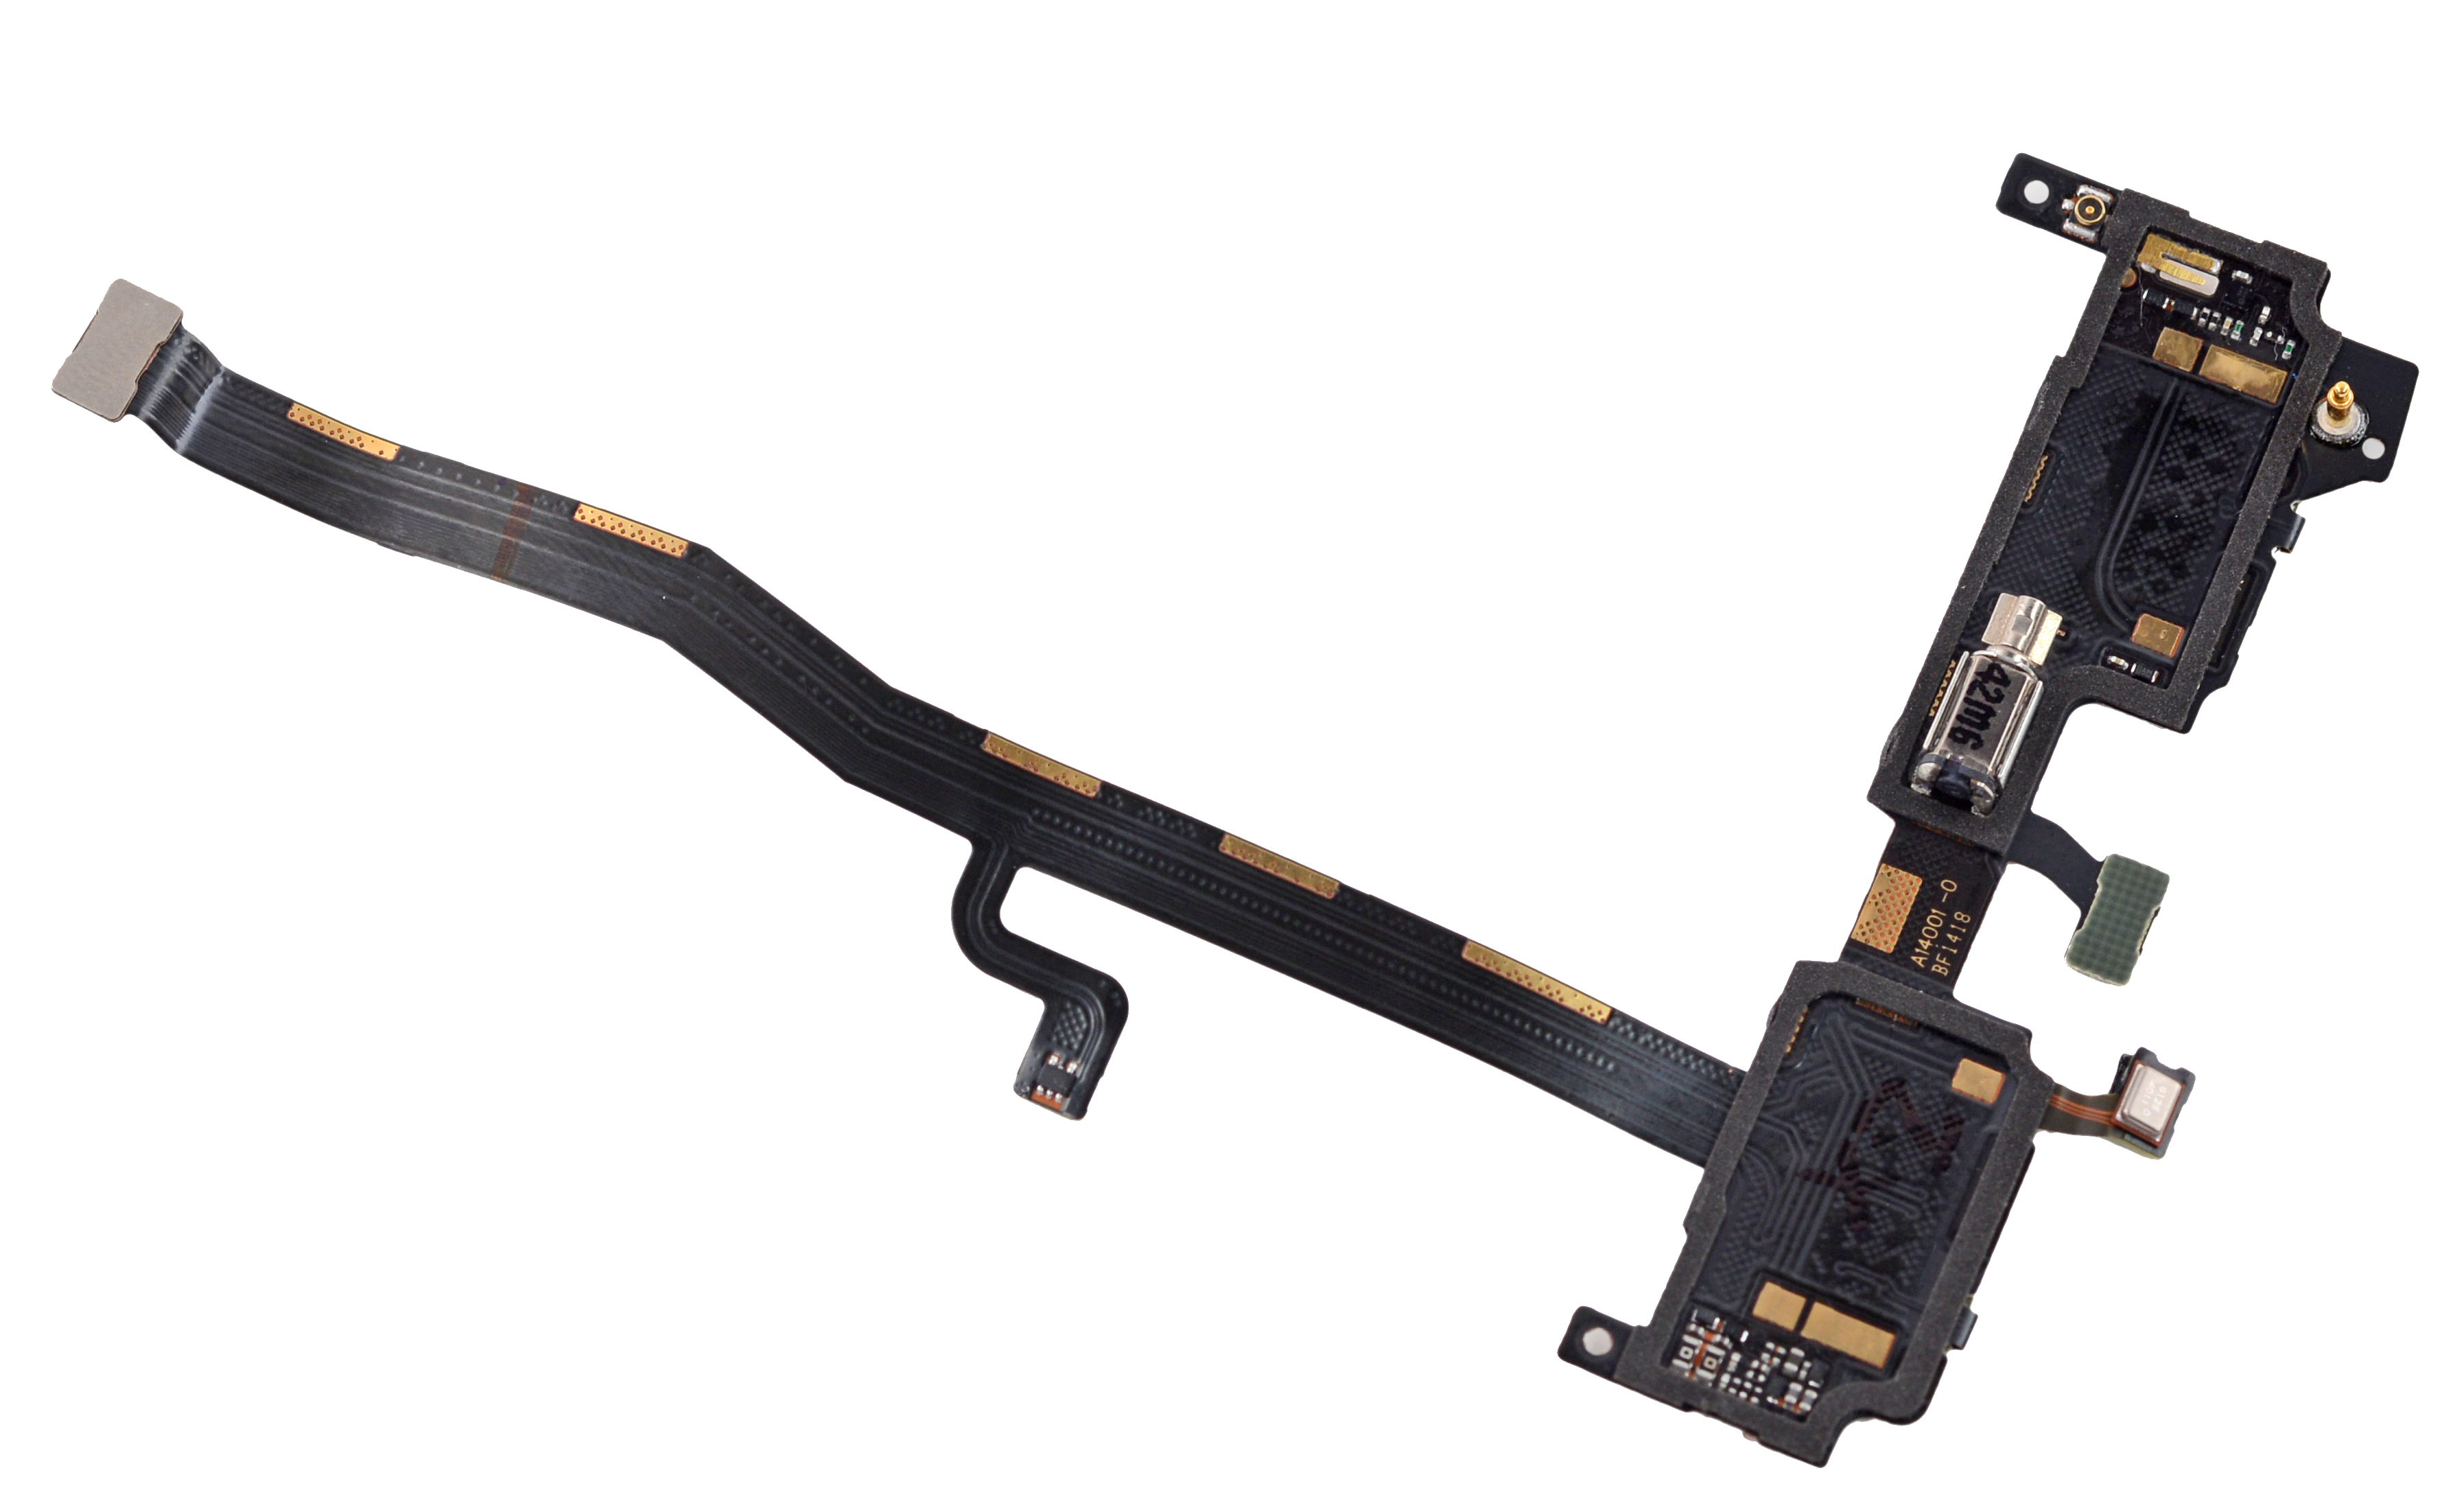
\includegraphics[width=\textwidth,height=6cm,keepaspectratio]{img/wdnGHA1UB3lBpZIL.png}
		\end{figure}
	\end{frame}    
%%%%%%%%%%%%%%%%%%%%%%%%%%%%%%%%%%%%%%%%%%%%%%%%%%%%%%%%%%%%%%%%%%%%%%%%%%%%%%%%%%%%



\section{Embedded System Components}	



%%%%%%%%%%%%%%%%%%%%%%%%%%%%%%%%%%%%%%%%%%%%%%%%%%%%%%%%%%%%%%%%%%%%%%%%%%%%%%%%%%%%
% About Sensors
%%%%%%%%%%%%%%%%%%%%%%%%%%%%%%%%%%%%%%%%%%%%%%%%%%%%%%%%%%%%%%%%%%%%%%%%%%%%%%%%%%%%
	\begin{frame}[t]{About Sensors}
		\small Sensors measure real-world phenomena and convert them into signals that we can process.	\\
		\vspace{0.5em}
		\begin{figure}
			\centering
			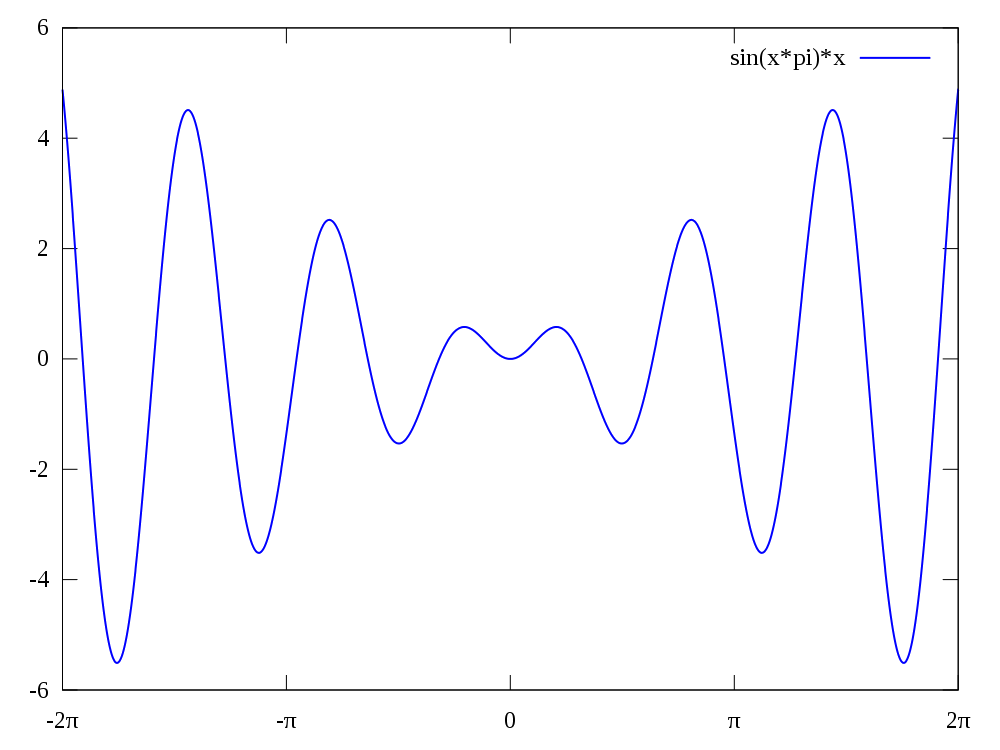
\includegraphics[width=\textwidth,height=0.6\textheight,keepaspectratio]{img/sine.png}
		\end{figure}
		Sensor results (in Volts, say) are continuous and analog...	\\	
		\hspace{2em}...but computers are discrete-time and digital. \\	
		\vspace{2em}		
		What to do? \\
	\end{frame}
%%%%%%%%%%%%%%%%%%%%%%%%%%%%%%%%%%%%%%%%%%%%%%%%%%%%%%%%%%%%%%%%%%%%%%%%%%%%%%%%%%%%



%%%%%%%%%%%%%%%%%%%%%%%%%%%%%%%%%%%%%%%%%%%%%%%%%%%%%%%%%%%%%%%%%%%%%%%%%%%%%%%%%%%%
% About Sensors
%%%%%%%%%%%%%%%%%%%%%%%%%%%%%%%%%%%%%%%%%%%%%%%%%%%%%%%%%%%%%%%%%%%%%%%%%%%%%%%%%%%%
\begin{frame}[fragile]{About Sensors}
\small{To convert an analog signal (e.g. voltage) to a digital value, we use an {\bf Analog-To-Digital Converter (ADC).}}	\\
\vspace{0.5em}
\begin{figure}[b]
\centering
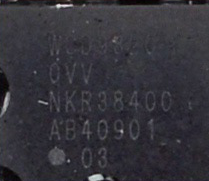
\includegraphics[width=\textwidth,height=4cm,keepaspectratio]{img/wcd9320_2.png}

\vspace{0.5em}
\begin{footnotesize}Qualcomm WCD9320 Audio CODEC from the OnePlus One\end{footnotesize}
\end{figure}
\end{frame}	
%%%%%%%%%%%%%%%%%%%%%%%%%%%%%%%%%%%%%%%%%%%%%%%%%%%%%%%%%%%%%%%%%%%%%%%%%%%%%%%%%%%%	
	
	
	
%%%%%%%%%%%%%%%%%%%%%%%%%%%%%%%%%%%%%%%%%%%%%%%%%%%%%%%%%%%%%%%%%%%%%%%%%%%%%%%%%%%%
% About Sensors
%%%%%%%%%%%%%%%%%%%%%%%%%%%%%%%%%%%%%%%%%%%%%%%%%%%%%%%%%%%%%%%%%%%%%%%%%%%%%%%%%%%%
\begin{frame}[fragile]{About Sensors}
\small To handle a continuous-time signal, we "sample" the signal at discrete times.	\\
\begin{tabular}{@{}m{0.5\textwidth} m{0.5\textwidth}@{}}
\begin{figure}
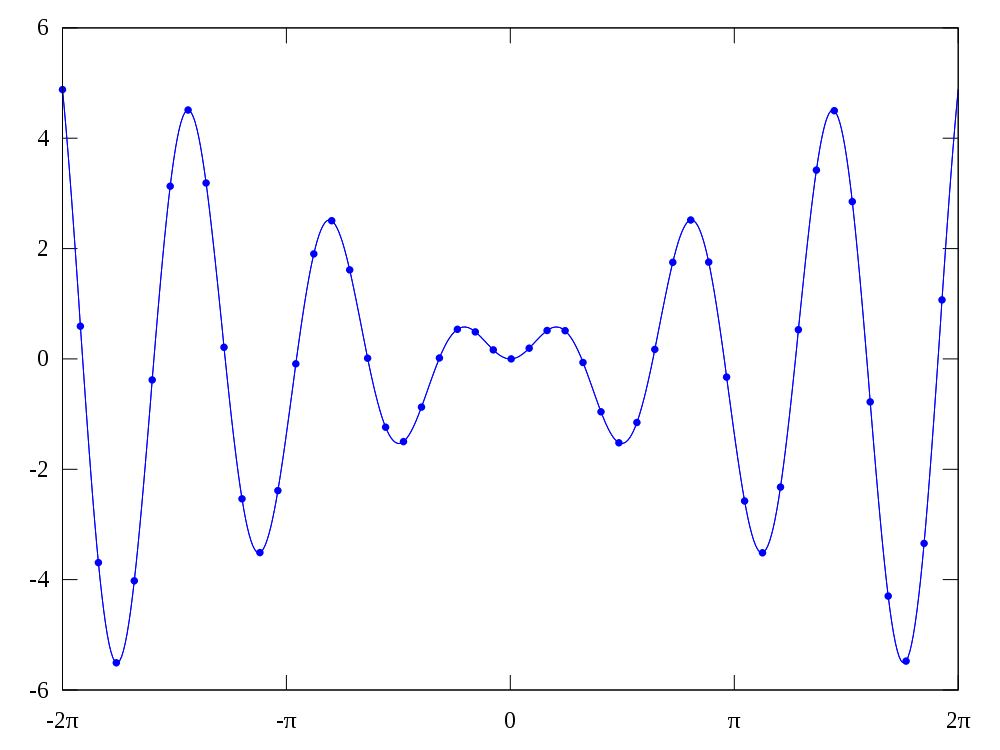
\includegraphics[height=0.65\textheight,keepaspectratio]{img/sine-points.png}
\end{figure}

&

\centering
\begin{tabular}{r|r}
Time (ms) & Signal (V) \\ \hline
0.0 & 0.00 \\
0.2 & 0.12 \\
0.4 & 0.38 \\
0.6 & 0.57 \\
0.8 & 0.47 \\
\end{tabular}
\end{tabular}
We lose information if samples too infrequent\footnote{Nyquist sampling theorem.}, or if sample resolution too poor. \\
\vspace{1em}
\end{frame}
%%%%%%%%%%%%%%%%%%%%%%%%%%%%%%%%%%%%%%%%%%%%%%%%%%%%%%%%%%%%%%%%%%%%%%%%%%%%%%%%%%%%



%%%%%%%%%%%%%%%%%%%%%%%%%%%%%%%%%%%%%%%%%%%%%%%%%%%%%%%%%%%%%%%%%%%%%%%%%%%%%%%%%%%%
% About Actuators
%%%%%%%%%%%%%%%%%%%%%%%%%%%%%%%%%%%%%%%%%%%%%%%%%%%%%%%%%%%%%%%%%%%%%%%%%%%%%%%%%%%%
\begin{frame}{About Actuators}
Actuators take signals from our embedded system and convert them into physical phenomena. \\
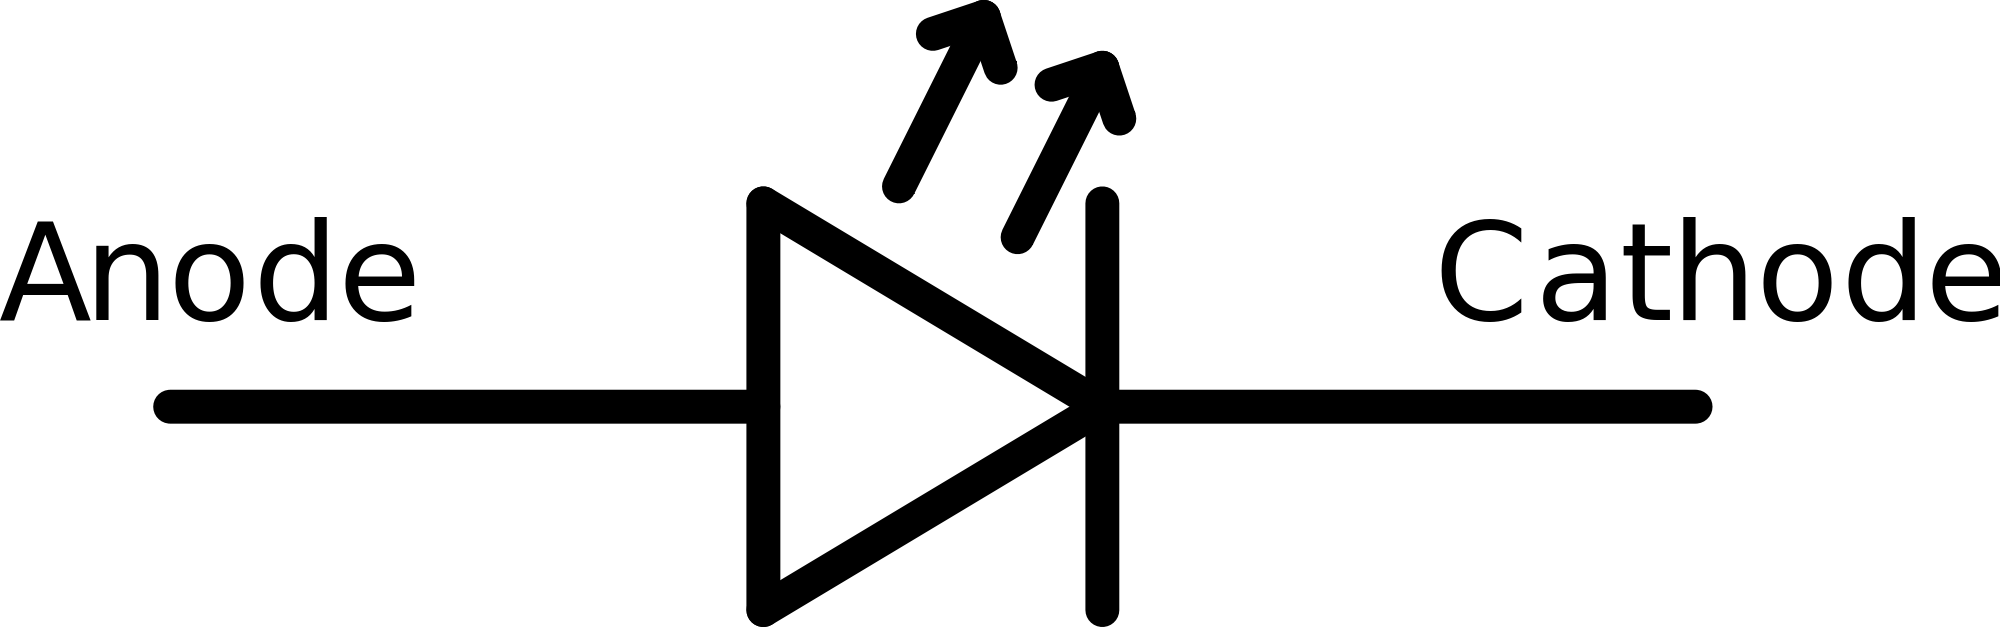
\includegraphics[scale=0.12,keepaspectratio,center]{img/2000px-LED_symbol.svg.png}
\begin{center}\begin{footnotesize}LEDs, the simplest of embedded actuators\end{footnotesize}\end{center} 
\vspace{2em}
What if our actuator requires an analog signal? We use a \textbf{Digital-to-Analog Converter (DAC)}. The audio CODEC we looked at has a DAC as well as an ADC.
\end{frame}  
%%%%%%%%%%%%%%%%%%%%%%%%%%%%%%%%%%%%%%%%%%%%%%%%%%%%%%%%%%%%%%%%%%%%%%%%%%%%%%%%%%%%

  
  
%%%%%%%%%%%%%%%%%%%%%%%%%%%%%%%%%%%%%%%%%%%%%%%%%%%%%%%%%%%%%%%%%%%%%%%%%%%%%%%%%%%%
% About Processing
%%%%%%%%%%%%%%%%%%%%%%%%%%%%%%%%%%%%%%%%%%%%%%%%%%%%%%%%%%%%%%%%%%%%%%%%%%%%%%%%%%%%  
\begin{frame}[t]{Processing}
\small
Programming an embedded system is somewhat different that a general-purpose computer. \\
\vspace{1em}
\begin{figure}
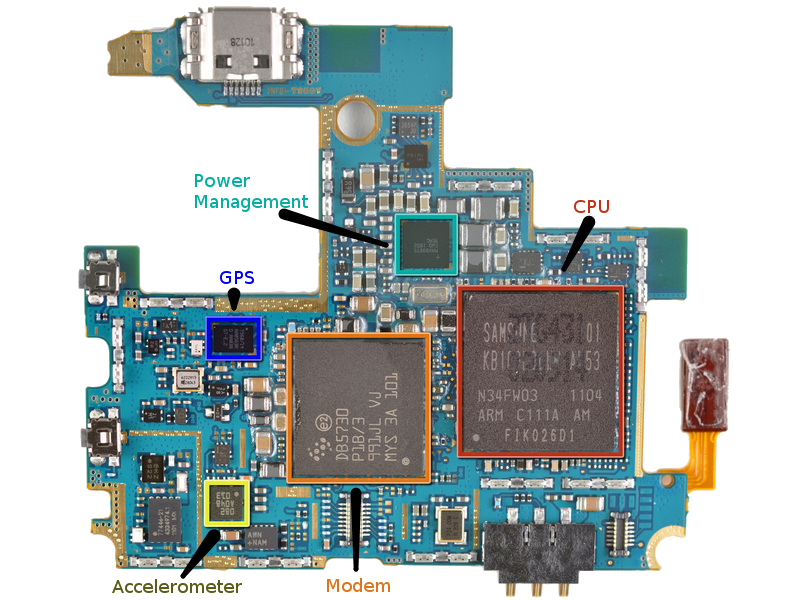
\includegraphics[width=\textwidth,height=0.6\textheight,keepaspectratio,left]{img/Galaxy_Logic_Board_Edited_2_small_annotated.png}
\captionsetup{justification=raggedright,singlelinecheck=false,labelformat=empty}
\caption{Samsung Galaxy S motherboard}
\end{figure}
\end{frame}
%%%%%%%%%%%%%%%%%%%%%%%%%%%%%%%%%%%%%%%%%%%%%%%%%%%%%%%%%%%%%%%%%%%%%%%%%%%%%%%%%%%%


  
%%%%%%%%%%%%%%%%%%%%%%%%%%%%%%%%%%%%%%%%%%%%%%%%%%%%%%%%%%%%%%%%%%%%%%%%%%%%%%%%%%%%
% Processing
%%%%%%%%%%%%%%%%%%%%%%%%%%%%%%%%%%%%%%%%%%%%%%%%%%%%%%%%%%%%%%%%%%%%%%%%%%%%%%%%%%%% 
\begin{frame}[t]{Processing}
\small
Programming an embedded system is somewhat different that a general-purpose computer. \\
\vspace{1em}
\begin{figure}
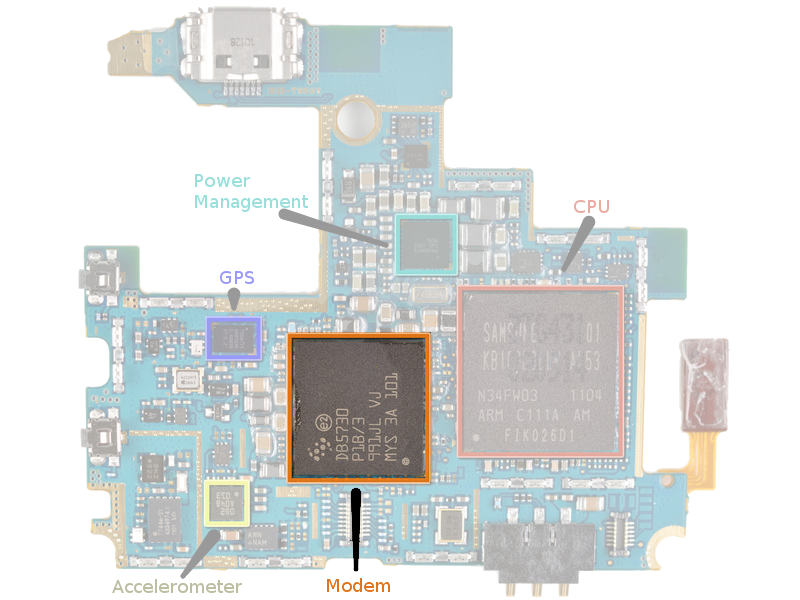
\includegraphics[width=\textwidth,height=0.6\textheight,keepaspectratio,left]{img/Galaxy_Logic_Board_Edited_2_small_annotated_highlight_modem.png}
\captionsetup{justification=raggedright,singlelinecheck=false,labelformat=empty}
\caption{Samsung Galaxy S motherboard}
\end{figure}
\end{frame} 
%%%%%%%%%%%%%%%%%%%%%%%%%%%%%%%%%%%%%%%%%%%%%%%%%%%%%%%%%%%%%%%%%%%%%%%%%%%%%%%%%%%%



%%%%%%%%%%%%%%%%%%%%%%%%%%%%%%%%%%%%%%%%%%%%%%%%%%%%%%%%%%%%%%%%%%%%%%%%%%%%%%%%%%%%
% Processing
%%%%%%%%%%%%%%%%%%%%%%%%%%%%%%%%%%%%%%%%%%%%%%%%%%%%%%%%%%%%%%%%%%%%%%%%%%%%%%%%%%%% 
\begin{frame}[t]{Processing}
\small
Programming an embedded system is somewhat different that a general-purpose computer. \\
\vspace{1em}
\begin{figure}
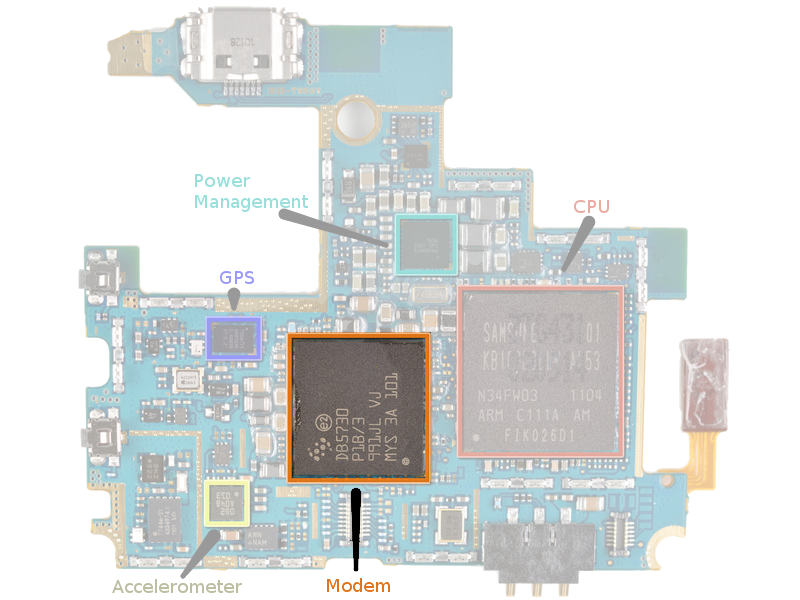
\includegraphics[width=\textwidth,height=0.6\textheight,keepaspectratio,left]{img/Galaxy_Logic_Board_Edited_2_small_annotated_highlight_modem.png}
\captionsetup{justification=raggedright,singlelinecheck=false,labelformat=empty}
\caption{Samsung Galaxy S motherboard}
\end{figure}
\putat{190}{60}{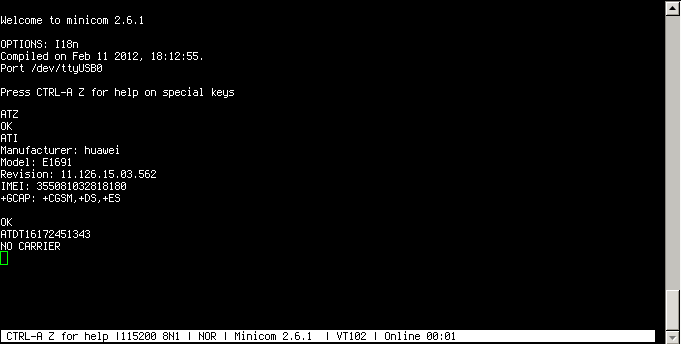
\includegraphics[scale=0.35]{img/modem-interaction.png}}
\end{frame} 
%%%%%%%%%%%%%%%%%%%%%%%%%%%%%%%%%%%%%%%%%%%%%%%%%%%%%%%%%%%%%%%%%%%%%%%%%%%%%%%%%%%%



%%%%%%%%%%%%%%%%%%%%%%%%%%%%%%%%%%%%%%%%%%%%%%%%%%%%%%%%%%%%%%%%%%%%%%%%%%%%%%%%%%%%
% Embedded Control Program
%%%%%%%%%%%%%%%%%%%%%%%%%%%%%%%%%%%%%%%%%%%%%%%%%%%%%%%%%%%%%%%%%%%%%%%%%%%%%%%%%%%% 
\begin{frame}{Running an Embedded Control Program}
The modem is running an \alert{embedded control program}.
\begin{itemize}
\item accepts high-level commands from the CPU;
\item translates bits into analog signals; contains ADC and DAC.
\end{itemize}

\vspace{1em}More generally, the modem:
\begin{itemize}
\item boots automatically,
\item never terminates,
\item translates stream of sensor inputs and actuator outputs,
\item cares about timing.
\end{itemize}
\end{frame}
%%%%%%%%%%%%%%%%%%%%%%%%%%%%%%%%%%%%%%%%%%%%%%%%%%%%%%%%%%%%%%%%%%%%%%%%%%%%%%%%%%%%



%%%%%%%%%%%%%%%%%%%%%%%%%%%%%%%%%%%%%%%%%%%%%%%%%%%%%%%%%%%%%%%%%%%%%%%%%%%%%%%%%%%%
% OnePlus One Modem
%%%%%%%%%%%%%%%%%%%%%%%%%%%%%%%%%%%%%%%%%%%%%%%%%%%%%%%%%%%%%%%%%%%%%%%%%%%%%%%%%%%%
\begin{frame}{What about the OnePlus One?}
Where's the modem in the OnePlus One? \\
\begin{figure}[b]
\centering
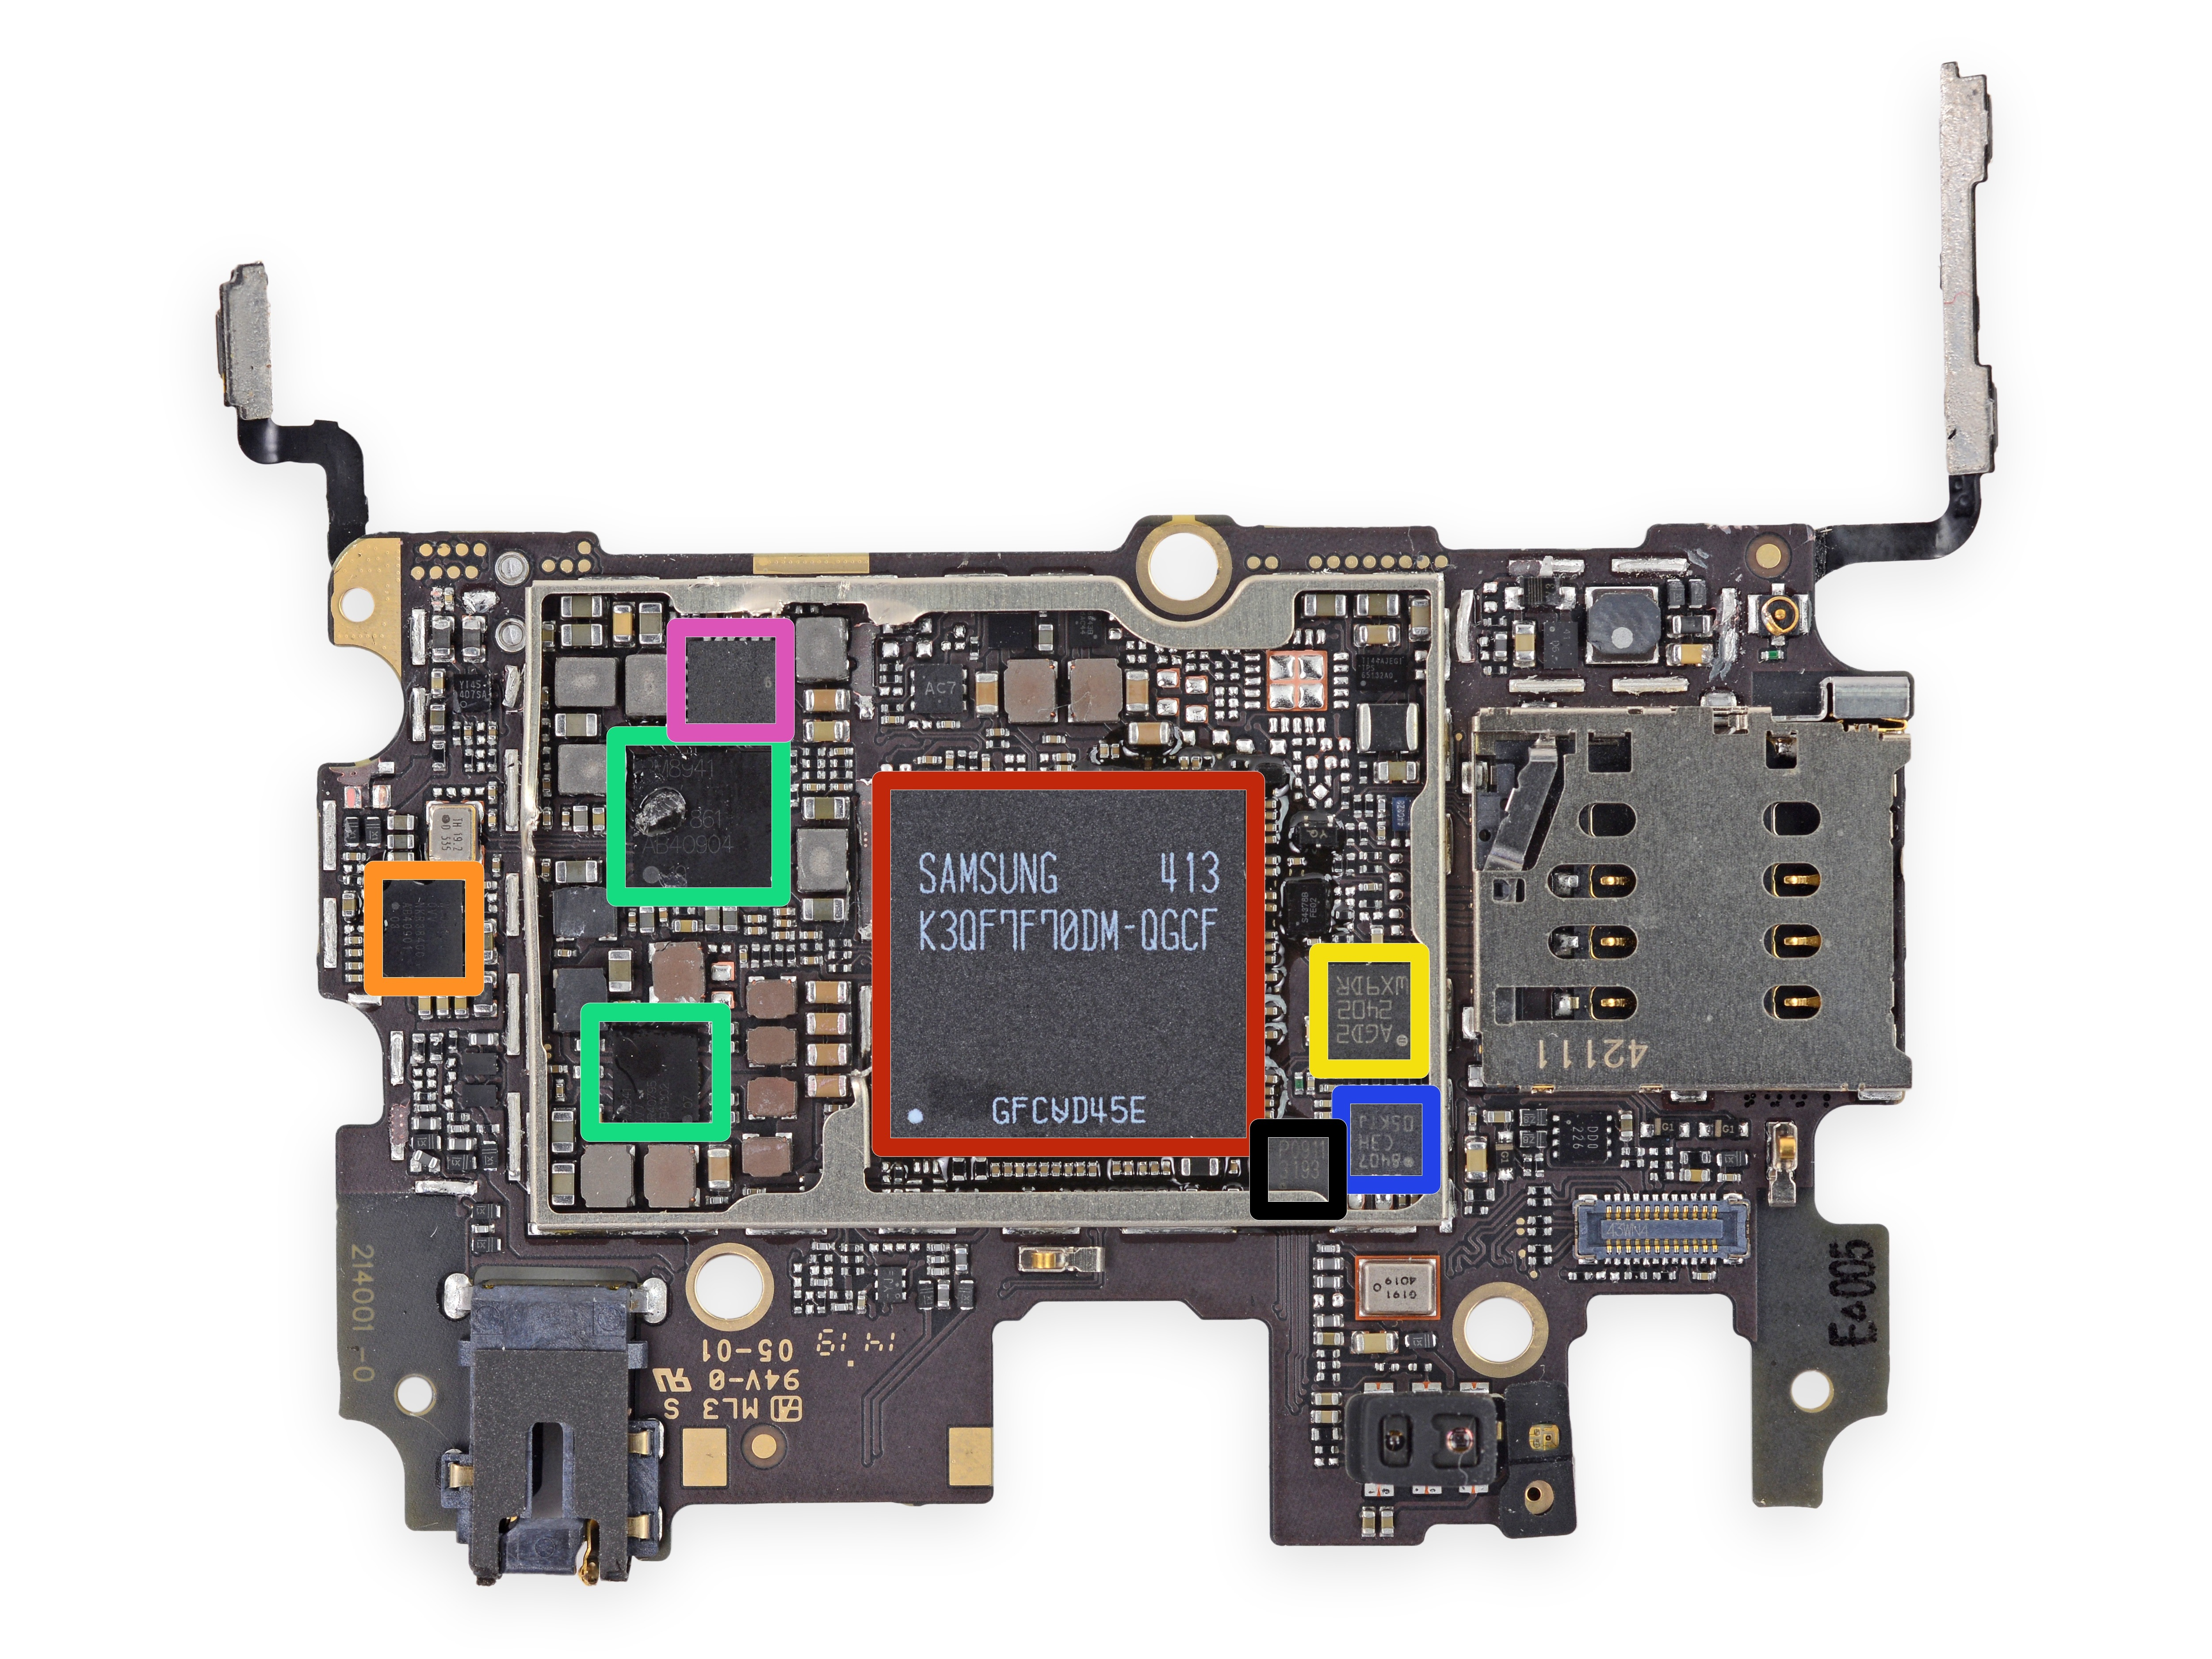
\includegraphics[width=\textwidth,height=6cm,keepaspectratio]{img/wIp5pQj4movpelpR.png}
\end{figure}
\end{frame}
%%%%%%%%%%%%%%%%%%%%%%%%%%%%%%%%%%%%%%%%%%%%%%%%%%%%%%%%%%%%%%%%%%%%%%%%%%%%%%%%%%%%



%%%%%%%%%%%%%%%%%%%%%%%%%%%%%%%%%%%%%%%%%%%%%%%%%%%%%%%%%%%%%%%%%%%%%%%%%%%%%%%%%%%%
% OnePlus One Modem
%%%%%%%%%%%%%%%%%%%%%%%%%%%%%%%%%%%%%%%%%%%%%%%%%%%%%%%%%%%%%%%%%%%%%%%%%%%%%%%%%%%%
\begin{frame}{What about the OnePlus One?}
Where's the modem in the OnePlus One? \\
\begin{figure}[b]
\centering
\includegraphics[width=\textwidth,height=6cm,keepaspectratio]{img/wIp5pQj4movpelpR_snappy.png}
\end{figure}
\end{frame}
%%%%%%%%%%%%%%%%%%%%%%%%%%%%%%%%%%%%%%%%%%%%%%%%%%%%%%%%%%%%%%%%%%%%%%%%%%%%%%%%%%%%



%%%%%%%%%%%%%%%%%%%%%%%%%%%%%%%%%%%%%%%%%%%%%%%%%%%%%%%%%%%%%%%%%%%%%%%%%%%%%%%%%%%%
% OnePlus One Modem
%%%%%%%%%%%%%%%%%%%%%%%%%%%%%%%%%%%%%%%%%%%%%%%%%%%%%%%%%%%%%%%%%%%%%%%%%%%%%%%%%%%%
\begin{frame}{What about the OnePlus One?}
\begin{figure}[b]
\centering
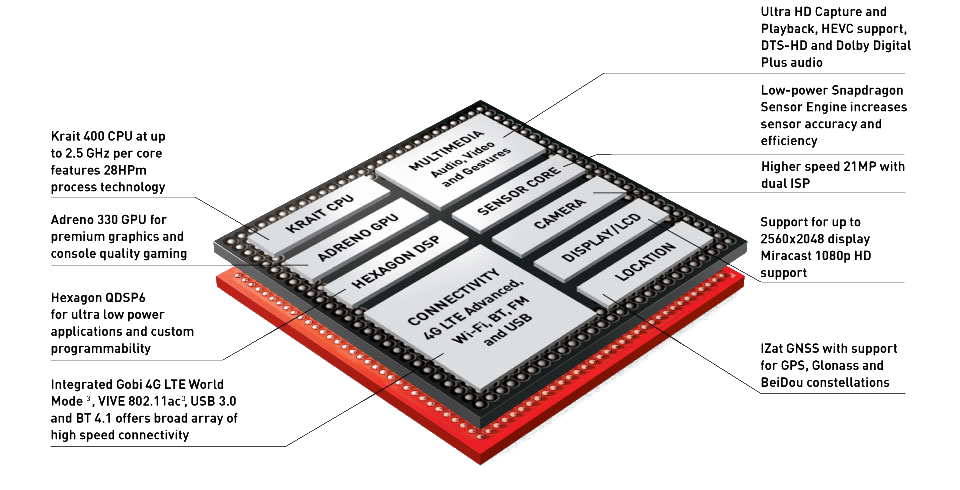
\includegraphics[width=\textwidth,height=6cm,keepaspectratio]{img/snapdragon-801-soc-image.png}
\captionsetup{labelformat=empty,font=scriptsize}
\caption{http://media.bestofmicro.com/V/9/427509/original/snapdragon-801-soc-image.png}
\end{figure}
\end{frame}
%%%%%%%%%%%%%%%%%%%%%%%%%%%%%%%%%%%%%%%%%%%%%%%%%%%%%%%%%%%%%%%%%%%%%%%%%%%%%%%%%%%%



%%%%%%%%%%%%%%%%%%%%%%%%%%%%%%%%%%%%%%%%%%%%%%%%%%%%%%%%%%%%%%%%%%%%%%%%%%%%%%%%%%%%
% Android
%%%%%%%%%%%%%%%%%%%%%%%%%%%%%%%%%%%%%%%%%%%%%%%%%%%%%%%%%%%%%%%%%%%%%%%%%%%%%%%%%%%%
\begin{frame}{Embedded Operating Systems: Android}
Android is an example of an \alert{embedded operating system}.\\[1em]
Target: smartphones and tablets.
\begin{itemize}
\item Runs Linux under the hood;
\item Using Java, insulates applications from the hardware;
\item Is compact and efficient;
\item Cares about battery life;
\item Favours portability;
\item Available under an open-source license (Apache).
\end{itemize}
We'll learn Android programming in this course.
\end{frame}
%%%%%%%%%%%%%%%%%%%%%%%%%%%%%%%%%%%%%%%%%%%%%%%%%%%%%%%%%%%%%%%%%%%%%%%%%%%%%%%%%%%%


\section{Safety and Embedded Systems}	



%%%%%%%%%%%%%%%%%%%%%%%%%%%%%%%%%%%%%%%%%%%%%%%%%%%%%%%%%%%%%%%%%%%%%%%%%%%%%%%%%%%%
% Therac-25
%%%%%%%%%%%%%%%%%%%%%%%%%%%%%%%%%%%%%%%%%%%%%%%%%%%%%%%%%%%%%%%%%%%%%%%%%%%%%%%%%%%%
\begin{frame}{Embedded Systems and Safety: Therac-25}
\centering
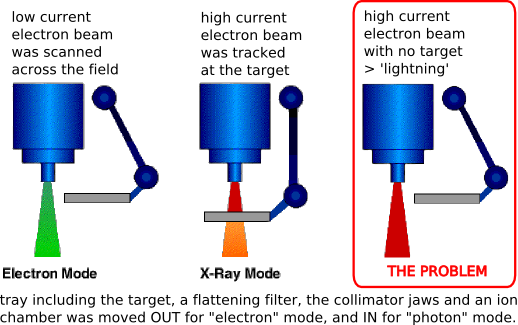
\includegraphics[width=0.65\linewidth,keepaspectratio]{img/Therac25.png}
\vspace{0.25em}
\begin{footnotesize}http://radonc.wikidot.com/local--files/radiation-accident-therac25/Therac25.png\end{footnotesize}
\end{frame} 
%%%%%%%%%%%%%%%%%%%%%%%%%%%%%%%%%%%%%%%%%%%%%%%%%%%%%%%%%%%%%%%%%%%%%%%%%%%%%%%%%%%%



%%%%%%%%%%%%%%%%%%%%%%%%%%%%%%%%%%%%%%%%%%%%%%%%%%%%%%%%%%%%%%%%%%%%%%%%%%%%%%%%%%%%
% Therac-25
%%%%%%%%%%%%%%%%%%%%%%%%%%%%%%%%%%%%%%%%%%%%%%%%%%%%%%%%%%%%%%%%%%%%%%%%%%%%%%%%%%%%
\begin{frame}{Embedded Systems and Safety: Therac-25}
  \begin{itemize}
  \item Radiation therapy machine
  \item Problem: \alert{many} $\rightarrow$ race conditions, overflow,
    no safety interlocks
  \item 3 patients died!
  \item Fix: software updates
  \end{itemize}

  \note[item]{\textbf{Problem Race Condition:} Race condition between
    the operator interface task and the equipment control
    task. Occurred only during quick controlling \textbf{(operator
      practice)}.}

  \note[item]{\textbf{Problem Overflow:} flag was incremented,
    overflow caused software to bypass safety checks.}

  \note[item]{\textbf{Problem Interlocks:} high-energy mode was
    enabled without target in place.}
\end{frame}
%%%%%%%%%%%%%%%%%%%%%%%%%%%%%%%%%%%%%%%%%%%%%%%%%%%%%%%%%%%%%%%%%%%%%%%%%%%%%%%%%%%%



%%%%%%%%%%%%%%%%%%%%%%%%%%%%%%%%%%%%%%%%%%%%%%%%%%%%%%%%%%%%%%%%%%%%%%%%%%%%%%%%%%%%
% Conclusion
%%%%%%%%%%%%%%%%%%%%%%%%%%%%%%%%%%%%%%%%%%%%%%%%%%%%%%%%%%%%%%%%%%%%%%%%%%%%%%%%%%%%
\begin{frame}[c]
  \frametitle{Conclusion}
  \textbf{\Large Someone has to build these systems!} \\
  Your life will depend on them.

  \pause

   \vspace{2em}
   Chances to learn about building safety-critical systems: \\
   \begin{itemize}
   \item ECE455 Embedded Software
   \item SE499: Independent project
   \item FYDP
   \item Undergraduate research assistant
   \end{itemize}
\end{frame}
%%%%%%%%%%%%%%%%%%%%%%%%%%%%%%%%%%%%%%%%%%%%%%%%%%%%%%%%%%%%%%%%%%%%%%%%%%%%%%%%%%%%

\end{document}